\documentclass{ioereport}
%\usepackage{lipsum} % Comment this if lorem ipsum is not needed

% The outlines in hyperrefs won't affect the printed documents so you can leave it as is
% \hypersetup{hidelinks}  % Uncomment to hide red-outlines in hyperreferences

\begin{document}
\newacronym{ai}{AI}{Artificial Intelligence}
\newacronym{ml}{ML}{Machine Learning}
\newacronym{nlp}{NLP}{Natural Language Processing}
\newacronym{api}{API}{Application Programming Interface}
\newacronym{bleu}{BLEU}{Bilingual Evaluation Understudy}
\newacronym{cnn}{CNN}{Convolutional Neural Network}
\newacronym{cv}{CV}{Computer Vision}
\newacronym{cpu}{CPU}{Central Processing Unit}
\newacronym{dsl}{DSL}{Domain Specific Language}
\newacronym{dslr}{DSLR}{Digital Single Lens-Reflex}
\newacronym{gui}{GUI}{Graphical User Interface}
\newacronym{html}{HTML}{Hyper Text Markup Language}
\newacronym{js}{JS}{JavaScript}
\newacronym{ldp}{LDP}{Line Drawing Prediction}
\newacronym{lstm}{LSTM}{Long Short Term Memory Networks}
\newacronym{mlp}{MLP}{Multi-layer Perceptron}
\newacronym{mp}{MP}{Mega Pixel}
\newacronym{relu}{RELU}{Rectified Linear Unit}
\newacronym{ui}{UI}{User Interface}
\newacronym{vit}{ViT}{Vision Transformer}
\newacronym{ann}{ANN}{Artificial Neural Network}
\newacronym{gpu}{GPU}{Graphic Processing Unit}
\newacronym{ln}{LN}{Layer Normalization}
\newacronym{css}{CSS}{Cascading Style Sheets}
\newacronym{rouge}{ROUGE}{Recall-Oriented Understudy for Gisting Evaluation}
\newacronym{ux}{UX}{User Experience}
\newacronym{ram}{RAM}{Random Access Memory}
\newacronym{json}{JSON}{JavaScript Object Notation}
\newacronym{ios}{iOS}{iPhone Operating System}
\newacronym{url}{URL}{Uniform Resource Locator}



% add the title preamble
\titlepreamble{Major Project Mid-term Report On}

% add the project title
\projecttitle{User Interface Code Generation from Hand-drawn Sketch} 

% add author names
\addauthor{Manoj Paudel}{THA077BCT025}
\addauthor{Prince Poudel}{THA077BCT036}
\addauthor{Ronish Shrestha}{THA077BCT040}
\addauthor{Sonish Poudel}{THA077BCT042}

% add supervisor name
\supervisor{Er. Devendra Kathayat}

% coverpage
\coverpage

% start of phantom section
\phantomsec

% for second coverpage
\coverpageB
\pagebreak

% Keep this section as it is
\iffalse 
\section*{DECLARATION}
    \addcontentsline{toc}{section}{DECLARATION}
    We hereby declare that the report of the project entitled \textbf{“\titlename”} which is being submitted to the \textbf{Department of Electronics and Computer Engineering, IOE, Thapathali Campus}, in the partial fulfillment of the requirements for the award of the Degree of Bachelor of Engineering in \textbf{Electronics, Communication and Information}, is a bonafide report of the work carried out by us. The materials contained in this report have not been submitted to any University or Institution for the award of any degree and we are the only author of this complete work and no sources other than the listed here have been used in this work.
    \\ \\ \\ \\
    \foreach \name [count=\i] in \authornames {
        \foreach \roll [count=\j] in \authorrollnumbers {
            \ifnum\i=\j
                \name\ (Class Roll No:\roll) \hrulefill \\ \\ 
            \fi 
        }
    }
    \\
    \textbf{Date:} \today
    \fi
    \pagebreak

% Only change the name, Keep this section as it is
\iffalse
\section*{CERTIFICATE OF APPROVAL}
    The undersigned certify that they have read and recommended to the \textbf{Department of Electronics and Computer Engineering, IOE, Thapathali Campus}, a major project work titled \textbf{``\titlename"} submitted by \textbf{\authornames} in partial fulfillment for the award of Bachelor's Degree in Computer Enginnering. The Project was carried out under special supervision and within the time frame prescribed by the syllabus.
    
    We found the students to be hardworking, skilled and ready to undertake any related work to their field of study and hence we recommend the award of partial fulfillment of Bachelor's Degree in Computer Enginnering.\\
    
    \rule{0.5\linewidth}{0.4pt}\\
    Project Supervisor\\
    \supervisorname\\
    Department of Electronics and Computer Engineering, Thapathali Campus\\

    \rule{0.5\linewidth}{0.4pt} \\
    External Examiner \\
    Prof. Dr. \textless Name of External\textgreater\\
    Department of Electronics and Computer Engineering, Pulchowk Campus\\

    \rule{0.5\linewidth}{0.4pt} \\
    Project Co-ordinator\\
    Er. \textless Name of Co-ordinator\textgreater \\
    Department of Electronics and Computer Engineering, Thapathali Campus\\

    \rule{0.5\linewidth}{0.4pt} \\
    Head of the Department \\ 
    Er. \textless Name of HOD\textgreater \\ 
    Department of Electronics and Computer Engineering, Thapathali Campus\\

    \today

    \pagebreak
    \fi

% Keep this section as it is
\iffalse
\section*{COPYRIGHT}
    The author has agreed that the Library, along with the Department of Electronics and Computer Engineering, Thapathali Campus, may make this report available for public inspection. Furthermore, the author has consented to the possibility of extensive copying of this project work for scholarly purposes, which may be granted by the supervising professor/lecturer or, in their absence, by the head of the department. It is understood that recognition will be given to the author and to the Department of Electronics and Computer Engineering, IOE, Thapathali Campus, for any use of the material from this report. Unauthorized copying for publication or other forms of financial gain without the express approval of both the Department of Electronics and Computer Engineering, IOE, Thapathali Campus, and the author is strictly prohibited.

    Requests for permission to copy or make any use of the material from this project, in whole or in part, should be addressed to the Department of Electronics and Computer Engineering, IOE, Thapathali Campus.

    \pagebreak
    \fi

\section*{ACKNOWLEDGMENT}
    \addcontentsline{toc}{section}{ACKNOWLEDGMENT}

    % Write Acknowledgements
We would like to express our sincere gratitude towards the Institute of Engineering,
Tribhuvan University for the inclusion of major project in the course of Bachelors in
Computer Engineering. We are also thankful towards our Department of Electronics
and Computer Engineering for the proper orientation and guidance during the project
\textbf{“User Interface Code Generation from Hand-drawn Sketch”}.

We would like to acknowledge the authors of various research papers and developers
of various programming libraries and frameworks that we have reference for
developing our project.
We would like to express our gratitude towards our Project Supervisor \textbf{\supervisorname} for continuous suggestions throughout.
Finally, we would like to thank all the people who are directly or indirectly related
during our study and preparation of this project.

    

    % Do not change this part
    Sincerely, 
    \par
    \par
    \def\namerolltable{}
    \foreach \name [count=\i] in \authornames {
        \foreach \roll [count=\j] in \authorrollnumbers {
            \ifnum\i=\j
                \xdef\namerolltable{\namerolltable \name & (Class Roll No:\roll) \\ \\} 
            \fi
        }
    }
    \begin{tabular}{@{}l@{\hspace{0.03\linewidth}}l@{}}
        \namerolltable
    \end{tabular} 



    \pagebreak

    
\section*{ABSTRACT}
    \addcontentsline{toc}{section}{ABSTRACT}

    % Write Abstract
This report presents “User Interface Code Generation from hand-drawn sketch” to
develop a machine learning-based system that can generate the code in HTML/CSS
from the given sketch of the layout. This project covers the topics of Image processing,
Transformer model, and compiler to translate the domain specific language to the
specific language on the basis of the platform. This system will be very useful to the
company that want to present the prototype of the user interface to the user. Our project
reduces the development time required to go from design to deployment. Skilled man
power in a company can focus on more complex and value adding aspect of the project.
Developers can easily customize and extend the generated code as per their need. We
can also add a dynamicity in the project by adding \gls{js} code. The system will
support multiple frontend frameworks providing flexibility and compatibility with
various development environment. The project is expected to develop a user-friendly
system that can generate code from the layout which can run on any platform.
    
    % Keywords in italics
    \textit{Keywords: Artificial Intelligence, \gls{dsl}, Image
Processing, Image synthesis, Self-Attention, Transformer Decoder, \gls{vit}}

    \pagebreak
    

% Table of Contents
\tableofcontents
\pagebreak

% List of Figures
\listoffigures
\pagebreak

% List of Tables
\listoftables
\pagebreak
  
% List of Abbreviations
\printglossary[type=\acronymtype,style=acronyms-only,title=List of Abbreviations{\vspace{0.5\baselineskip}}]
\pagebreak
% end of phantom section


% Start of main section
\mainsection

\section{\MakeUppercase{Introduction}}

    \subsection{Background}
In realm of software development process traditionally user interface development has
been relied on manual interpretation and implementation of design specifications.
Although, manual coding of UI elements such as buttons, input fields, and layouts
consumes not only valuable time but also introduces multiple potential errors and
variations between the intended design and the implemented interface. Upon
discovering the fact this project aims to address these challenges by proposing a system
Sketch-to-code, capable of transforming sketches into executable front-end code. It
addresses the challenges that have been affecting designers and developers for years:
that even though designers go to great lengths to create digital solutions that are
perfectly measured and consistently crafted, design systems do not fluently translate to
development systems.

In recent years, technology and \gls{ai} have significantly changed the
process of converting \gls{gui} sketches into functional frontend
code. Researchers are exploring machine learning and advanced image processing to
develop automated systems capable of understanding and generating code directly from
design sketches. These systems benefit developers by speeding up UI development,
ensuring consistency between design and implementation, and allowing for more focus
on refining user experience and functionality. Furthermore \gls{ai}-driven solutions
continue to advance, they promise to revolutionize software development practices,
making them more efficient and accessible for developers across different industries.
    \subsection{Motivation}
This project aims to solve a common problem in software development: the lengthy
process of turning design ideas into working software. Developers often face challenges
when the final product doesn't match the original design, which leads to making many
adjustments and can cause delays in finishing projects on time. In order to solve this
problem, we will be providing simple prototype front end code which will be easier for
developer. By automating the first steps of creating user \gls{ui} , we want to
make this process faster and smoother. This means developers can spend more time improving how the software works for users, rather than getting stuck on the technical
details of building buttons and menus.

In essence, our goal is to use technology to simplify software development, making it
easier for developers to create software that matches the original vision without wasting
time on repetitive tasks. Moreover, not to create variance from the original intended
design of user.
    \subsection{Problem Definition}
The problem is to develop a system that can automate the process of turning sketches
into functional front-end code. The system should be able to craft interactive \gls{ui} that is more like designer intended.

Some of the key challenges are listed below:

\begin{itemize}
    \item \textbf{Ambiguity in Requirements:} Sketches may not always clearly define all
    requirements, leading to ambiguity. This can result in misunderstandings
    between stakeholders, designers, and developers.
    \item \textbf{Technical Feasibility:} Sometimes, what looks good on paper (or screen) may
    not be technically feasible within the constraints of the project, platform, or
    technology stack. 
    \item \textbf{Integration Complexity:} Projects often require integrating various
    components, APIs, or third-party services, which can introduce complexity
    beyond the initial sketch.
    \item \textbf{\gls{ux} Considerations:} Implementing a sketch into code
    involves not just visual fidelity but also ensuring a smooth and intuitive user
    experience, which may require iterative improvements.
\end{itemize}
    \subsection{Objectives}
    The main objectives of our project are listed below :
    \begin{itemize}
        \item To construct a model able to generate quick \gls{gui} prototype
        \item To make intutive user interface for customizing and stylizing the generated
code.
    \end{itemize}
    
    \subsection{Project Scope and Applications}
    \sloppy
    Computer science projects typically start with a concept or idea, often visualized 
    through sketches or diagrams that outline the project's goals, user interfaces, and system
    architecture. These sketches serve as a blueprint for translating abstract concepts into
    tangible software solutions. The scope of converting these sketches into code lies in
    transforming visual representations into functional code that aligns with specific
    requirements and user needs.
    \unskip
    

The application of this sketch-to-code transition simplifies the development process by
providing a clear roadmap for programmers to follow. It ensures that developers
understand the project's scope, functionalities, and design aesthetics from the outset.
By adhering to the sketches, developers can maintain consistency in design elements,
streamline development iterations, and effectively manage project timelines and
resources. Moreover, the sketches serve as a communication tool between stakeholders,
designers, and developers, fostering collaboration and alignment throughout the project
lifecycle.

In practical terms, the transition from sketches to code involves selecting appropriate
programming languages, frameworks, and tools that best fit the project's requirements.
Developers interpret the visual concepts into code syntax, ensuring that each
component functions as intended and integrates seamlessly with other project modules.
This process demands attention to detail, problem-solving skills, and a keen eye for
user experience to deliver software that not only meets technical specifications but also
provides a user-friendly interface.

Furthermore, the sketches-to-code approach facilitates iterative development and agile
methodologies, allowing for continuous feedback and improvement based on user
testing and stakeholder input. It empowers developers to make informed decisions,
address challenges promptly, and adapt to evolving project requirements. Ultimately,
by translating project sketches into code effectively, computer science projects can
achieve their objectives efficiently, delivering robust software solutions that meet both
technical standards and user expectations.
    \pagebreak
    
\section{\MakeUppercase{Literature Review}}
    \subsection{Different methods used for this kind of task}
    For the survey, databases like IEEE Xplore , Google Scholar, and Articles were
searched manually, by using various keywords like “sketch to code”, “pics to code”,
”Image to functional code” etc. Research papers of various paper were shown on the
search from the mentioned repositories like Journals, Conferences and Articles. Along
with Research papers, certain existing systems were also reviewed. The research paper
were studied and then this literature review explores the key methodologies, tools and
technologies that have been developed and the progress made in this domain. In 2017, Pix2code is an system described in the paper "Generating Code from a
\gls{gui} Screenshot.Pix2code is a technology that converts \gls{gui} designs, like screenshots, into executable code. Developed using
deep learning techniques, it analyzes the visual layout of buttons, menus, and other
elements to generate corresponding code in various programming languages. This
innovation bridges the gap between design and development by automating the
translation of visual concepts into functional software components. By interpreting the
structure and properties of each \gls{gui} element, Pix2code ensures accuracy in code
generation, speeding up the prototyping and development process significantly. This
approach not only enhances efficiency but also facilitates collaboration between
designers and developers, making it easier to translate design ideas into tangible
applications seamlessly. \cite{beltramelli2017pix2codegeneratingcodegraphical}

In 2019, the paper titled “Eve: A sketch-based Software Prototyping Workbench”
presents a novel approach to transforming hand-drawn sketches into software
prototypes. Prototyping involves the evolution of an idea into various stages of design
until it reaches a certain level of maturity. Conventional approaches to software
prototyping typically involve Manual Coding, Graphic Design Tools \& Hybrid
Approaches. However they did it through a process wise approach which includes User
Interface Sketch Recognition, \gls{ml}, Prototype Generation, and User
Interaction and at the end Feedback Loop. They present a promising approach to
automating the translation of hand-drawn sketches into interactive software prototypes by streamline the prototyping process. However the system faces challenges related to
recognition accuracy, complexity handling, scalability, usability and integration. \cite{10.1145/3290607.3312994}

In 2020, the paper titled "Automatic Code Generation from Low Fidelity Graphical
User Interface Sketches Using Deep Learning" explores an advanced method for
converting hand-drawn, low-fidelity \gls{gui} sketches into functional code using deep
learning techniques. The process involves cleaning the sketches, recognizing different
\gls{ui} components using neural networks, and then generating the corresponding code with
models designed for handling sequences, like \gls{lstm}. Specifically, it uses
\glossary{cnn} for image recognition and \gls{lstm} networks for sequence prediction, enhancing the system's ability to
accurately interpret and generate code from sketches. The combination of CNNs for
detailed image analysis and \gls{lstm} for managing sequential data allows the system to
better handle complex and densely packed \gls{ui} layouts. This is an improvement over
simpler models that struggled with intricate designs. This approach aims to make \gls{ui}
design faster and more efficient, but it faces challenges such as accurately interpreting
diverse sketch styles, managing complex layouts, and ensuring the generated code
integrates well with existing development workflows. \cite{9971204}

Moreover, the paper "Automatic Code Generation from Sketches of Mobile
Applications in End-User Development Using Deep Learning" presents a system that
allows users to sketch mobile app interfaces, which are then automatically converted
into functional code using deep learning techniques. This approach aims to democratize
app development by enabling users without programming skills to create applications.
The system utilizes \gls{cnn} for accurate recognition
of UI elements and \gls{lstm} networks for generating
corresponding code sequences. Despite advancements, challenges such as ensuring
accuracy across diverse sketch styles and integrating seamlessly into existing
development workflows remain. Overall, the research marks a significant step towards
empowering end-users in mobile app creation through automated code generation from
conceptual sketches. \cite{Baule2021}

Similarly, in 2024 a paper was published in IEEE, STC (Sketch To Code)-An Enhance Html \& CSS Autocode Generator from Handwritten Text and Image Using Deep Learning. The authors unfolds in four distinct phases: Pre-processing, Segmentation,
Feature Extraction employs \gls{ldp} for detailed interpretation
and Classification Categorizes features into \gls{html} and \gls{css} elements. Early
approaches relied heavily on rule-based systems and heuristics. These methods
involved predefined templates and rules to convert sketches into code. However, these
systems were inflexible and struggled with complex or unconventional sketches. \cite{10537336}
\subsection{Vision Transformer for Computer vision}
Dosovitskiy et al. proposed the vision transformer, which can take image as an input
and process it to classify the image at their paper “An Image is worth 16 x 16 words:
Transformers for Image Recognition at scale”. Transformer have gained popularity in
\gls{cnn} and to extend this concept in \gls{cv}, they
designed this transformer model. \cite{dosovitskiy2021imageworth16x16words}
    \pagebreak

\section{\MakeUppercase{Requirement Analysis}}
    \subsection{Software Requirement}
    \subsubsection{Python}
    Python is a high level, versatile and user-friendly general purpose, dynamic
programming language where multiple programming paradigms, including objectoriented, imperative and functional programming are supported. It is an open source
programming language, which let us work quickly and integrate system easily.
\subsubsection{Numpy}
Numpy stands for Numerical Python. Numpy is a package to perform numeric
programming extension for python. It is the core library to compute scientific
calculation in python. Numpy provide an array object which is up to 50x faster than
traditional python lists.
\subsubsection{Tensorflow}
Tensorflow is basically defined as a open source software library, developed by google
for various numerical computation using data flow. Tensorflow is used for building and
training deep learning models, facilating the creation of computational graphs and
efficient execution on various hardware platforms.
\subsubsection{Keras}
Keras is an open source library that offers a python interface for \gls{ann} and acts as interface to TensorFlow library. Keras acts as host tools to
simplify programming language in deep neural network area while working with texts
and images data. Keras is implemented in various neural-network building block area
such as layers, optimizers and activation functions
\pagebreak
    \subsection{Hardware Requirement}
    \subsubsection{Camera device}
    To collect the image of manually sketch design of paper any mobile phone with camera
of minimum of 12 \gls{mp} is required. More than 12 \gls{mp} camera phone or may be \gls{dslr}
camera will be additionally fruitful for us to capture high resolution images.
    \subsubsection{Cloud Computing Platform}
    For the training purpose of our model, it is essential for us with a dedicated \gls{gpu} and
\gls{cpu} with sufficient capacity of \gls{ram}. For training purpose, we will be using colab or
kaggle GPU platform, which both provide us a free hosted jupyter notebook
environment in the cloud.
    \pagebreak
    
\section{\MakeUppercase{System Architecture and Methodology}}
\subsection{Dataset}
Our approaches require a dataset which contains a wireframe sketch and associated
\gls{dsl} code. Sourcing a quality dataset is often a challenge in many machine learning
projects. We were not aware of any dataset which contained wireframes sketches and
associated \gls{dsl} code, and therefore created our own.
\subsubsection{Dataset Generator}
The dataset generator is a crucial component of our project, designed to create a large
and diverse set of training samples for our model. It operates through a multi-step
process that begins with the random generation of \gls{dsl}
code, which describes the structure and elements of a web page layout. This \gls{dsl} code
is then compiled into HTML and CSS, which is subsequently rendered to create a visual
representation of the layout. Then, it is analyzed to identify the positions and outlines
of various elements. In the final step, hand-drawn sketches are placed of the elements
at the appropriate position, then we get a sketch corresponding to the original \gls{dsl} code.
This automated process allows us to rapidly produce a large number of sketch-\gls{dsl}
pairs, each unique and representative of real-world web designs. The generator used the
predefined rules and constraints which ensures that the produced layouts are diverse
and realistic. This approach helps in addressing the challenges of requiring lot of dataset
while training the model.
\begin{figure}[H]
    \centering
    \includegraphics[width=\textwidth]{images/Dataset Generator.png}\caption{Block Diagram of Data Synthesis}\label{fig:Synthesis}
\end{figure}



    \subsection{Block Diagram}

 \begin{figure}[H]
        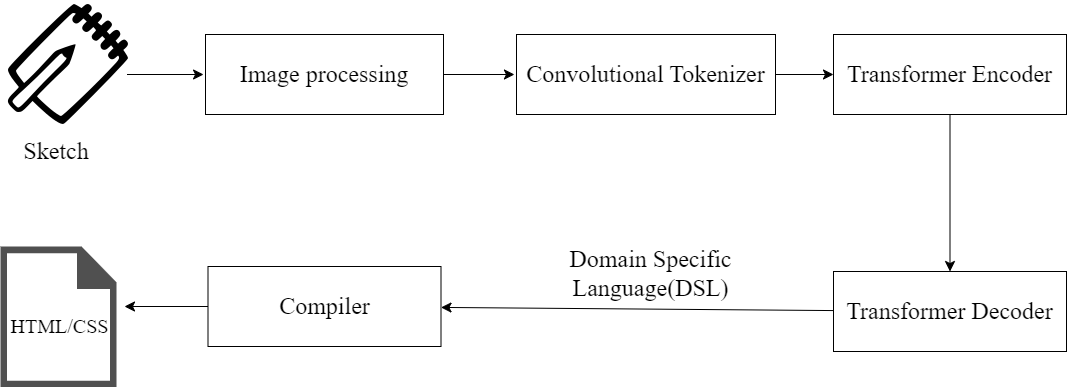
\includegraphics[scale=5]{images/Block Diagram.png}
        \caption{Block Diagram of Working of System}
        \label{fig:block}
    \end{figure}

    \subsection{Working Principle}
    The input data for this project is the sketch of the UI. The sketch is transformed to the
HTML code. It involves following steps:
\begin{itemize}
    \item \gls{dsl} code extraction using Transformer model
    \item Compiling \gls{dsl} code to HTML code
\end{itemize}
\subsubsection{Image Processing}
Preprocessing is required to translate an image from a camera into an image which can
be fed into the model. Due to the positioning of the camera or lighting conditions the
raw image must be cleaned up before it can be processed.

The main challenges are:
\begin{itemize}
    \item The image may not fill the entire frame, as such the background must be
removed. 
    \item The paper may be skewed or rotated.
    \item The image may contain noise or alterations due to lighting.
\end{itemize}

For solving above challenges:
\begin{itemize}
    \item We will detect the paper in the image and crop it. As our requirements state that
the medium must be white, to detect the paper we converted the image to HSV
and used threshold filtering to remove all colors except white. This process
reduces the background noise considerably. As the paper contains the sketch in
a dark marker, these pixels will be filtered by the threshold filtering. As such,
to fill the gaps left by the sketch we will apply a large median blur. We will
apply canny edge detection and dilated the edge map to close small gaps
between the edges. Finally, we will apply contour detection and find the largest
contour with approximately four sides (as we assume the medium is four sided
e.g. paper or a white board).
removed. 
    \item We will use perspective warping to unwrap the four corners of the contour found
and map them to an equivalent rectangle for correcting the orientation of the
page.
    \item We will apply a median blur to the unwrapped cropped image to reduce noise.
We then ran Canny edge detection and dilated the edge map to close small gaps
between lines. The result of the post processing is an unskewed binary edge map
of the sketch. This is fed into our model for processing
\end{itemize}
\textbf{Canny Edge Detection Algorithm}
The process of canny edge detection algorithm can be broken down to five different
steps: 
\begin{enumerate}
    \item Apply Gaussian filter to smooth the image in order to remove the noise
    \item Find the intensity gradients of the image
    \item Apply gradient magnitude thresholding or lower bound cut-off suppression to
get rid of spurious response to edge detection
    \item Apply double threshold to determine potential edges
    \item Track edge by hysteresis: Finalize the detection of edges by suppressing all the
other edges that are weak and not connected to strong edges.
\end{enumerate}
\subsubsection{Convolutional Tokenizer}
A convolutional tokenizer is a neural network component that processes image inputs
using convolutional layers to create a sequence of tokens. A convolutional tokenizer
works on visual data. It applies a series of convolutional filters across the image,
capturing local patterns and features at different scales. These convolutional operations
are typically followed by pooling layers, which reduce spatial dimensions while
retaining important information. The result is a set of feature maps that represent highlevel abstractions of the input image. These feature maps are then flattened or reshaped
into a sequence of vectors, where each vector can be considered a "token" representing
a specific part or feature of the image. This process bridges the gap between image data
and sequence models, allowing techniques from natural language processing to be
applied to visual tasks.
\subsubsection{Transformer Model}
Transformer model is used to generate structural description of the image in the form
of \gls{dsl} code. Transformer is a deep learning architecture that consists of encoderdecoder structure. The transformer processes input sequence of tokens to sequence of
continuous representation. Given the output representation of the encoder, then the
decoder generate output sequence of symbols. The transformer model consists of
stacked self-attention and fully connected layer for both encoder and decoder.Our project works similar to the image captioning. In the Image captioning model, input
is the image and the output is the text describing the image. Whereas in our model, it
will give a structural description of the interface as output in Domain Specific language.


    \begin{figure}[H]
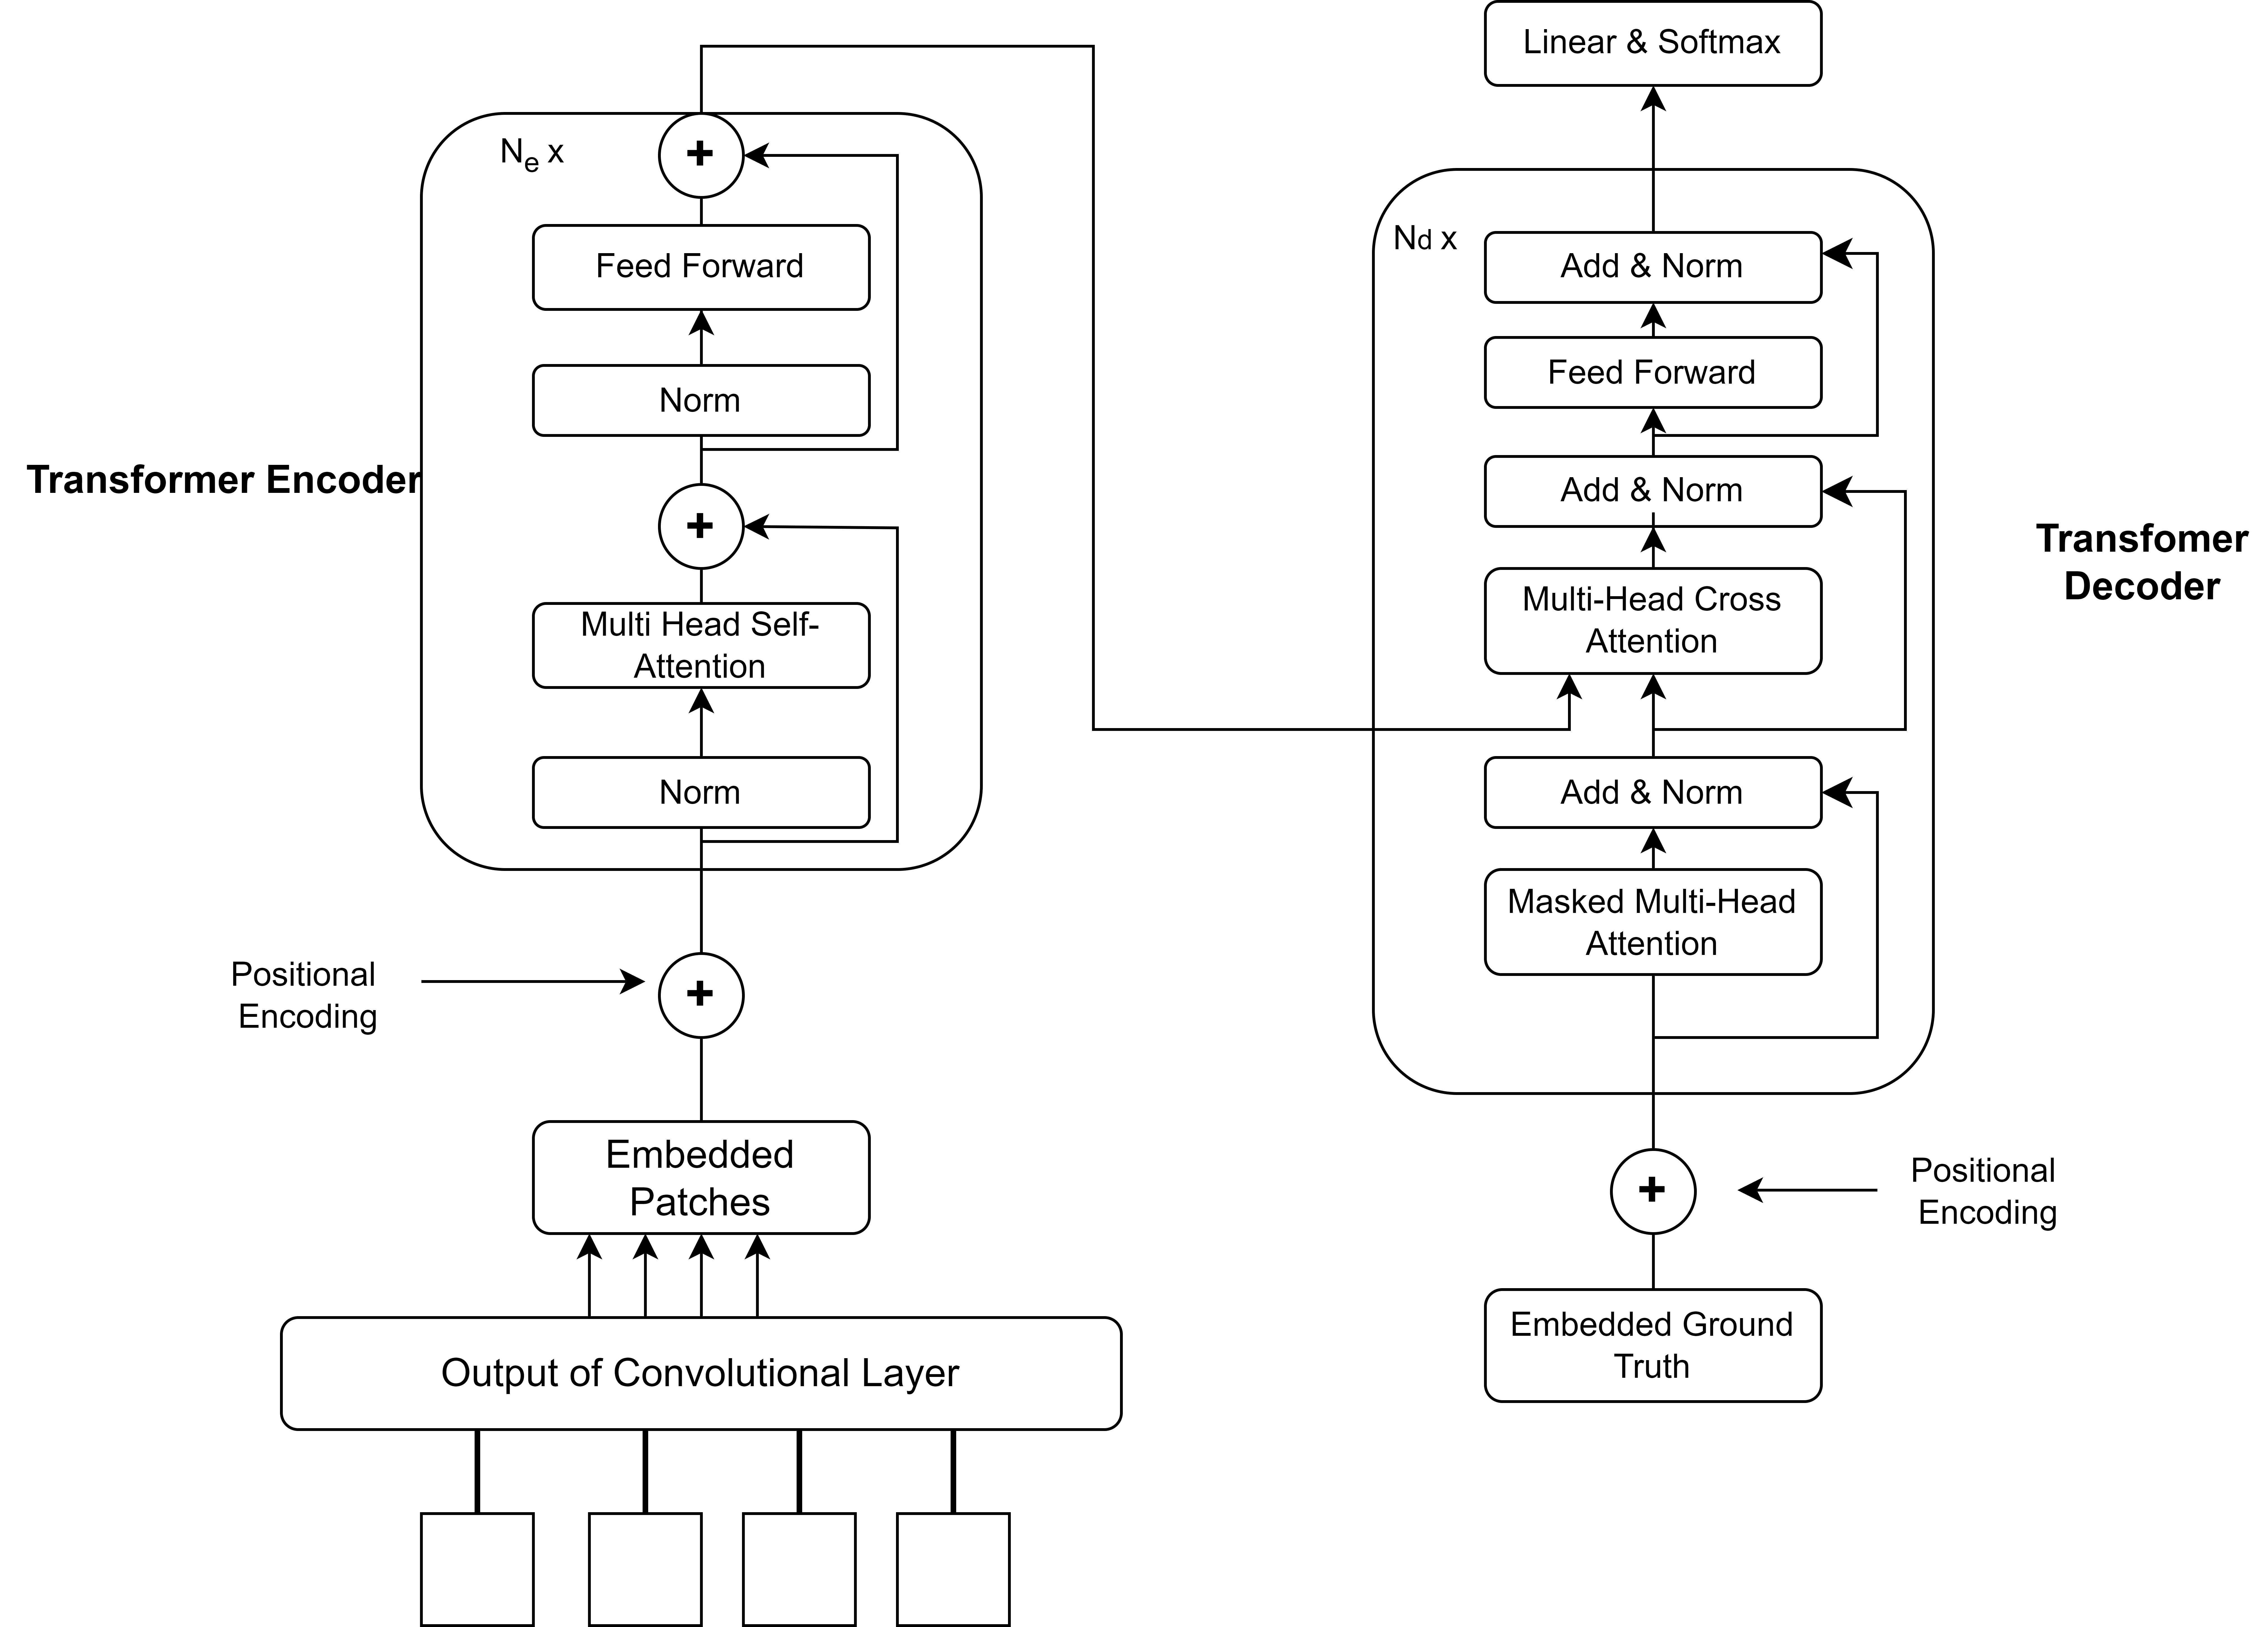
\includegraphics[scale=.7]{images/Transformer.png}
\caption{Block Diagram of Transformer Model}
\label{fig:transfor}
\end{figure}
\textbf{Transformer Encoder}\\
The transformer encoder is a key component of the transformer architecture which is
originally designed for \gls{nlp} tasks. Now, it is widely used in various domains, including
\gls{cv}. It consists of multiple identical layers, each containing two main sublayers: a multi-head self-attention mechanism and a position-wise fully connected feedforward network. The self-attention mechanism allows the model to weigh the
importance of different parts of the input sequence when processing each element,
enabling it to capture complex dependencies regardless of their distance in the
sequence. The feed-forward network processes each position independently, adding
non-linearity and increasing the model's capacity to learn complex functions. Layer
normalization and residual connections are employed around each sub-layer to facilitate
training of deep networks.\\
\textbf{Transformer Decoder}\\
The transformer-based decoder consists of Nd stacked identical transformer block
similar to the encoder. Each transformer decoder block is composed of a masked multihead self-attention sublayer followed by a multi-head cross attention sublayer and a
positional feed-forward sublayer sequentially. The decoder in our model takes in the
encoded image embeddings and the embedded ground truth caption sequences. In
addition, we add positional embedding to it for word embedding features, which is
added to make use of the order of the ground truth caption sequences. The positional
encodings have the same dimension as the sequence embeddings to be summed. The
decoder block utilizes the last decoder block’s output feature to predict the next word
via a linear layer whose output dimension equals the vocabulary size.\\
\textbf{Attention}\\
Attention can be describe as a similarity between the query and key. They take the form:
\begin{equation}
\text{Attention}= \text{similarity}(q, k)
\end{equation}
Where q represents a query and k represents a key. It’s like accessing a database, where
we query the database looking for the information we want. To find the similarity
between queries and keys, dot product is normally used. It provide the value between 0
and 1. If they are different, obtained value is 0 otherwise it is 1. The output is computed
as a weighted sum of the values, where the weight assigned to each value is computed
by a compatibility function of the query with the corresponding key.\\
\textbf{Self-Attention}\\
In order to identify dependencies and relationships within input sequences, selfattention is a method employed in machine learning, especially in natural language
processing and \gls{cv} applications. By taking care of itself, the model is able
to recognize and assess the relative value of various input sequence components. In
self-attention, vector q, k, v which are actually neural networks (typically linear) have
same input (q(x), k(x), v(x)), then they are self- attending.\\
\textbf{Scaled Dot-Product Self-Attention}\\
Here, the dimensionality of queries and keys are denoted by dk and dimensionality of
values is denoted by dv. The scaled dot-product attention then receives these queries,
keys, and input values and computes the dot-product of the queries with the keys. The
attention scores are then obtained by scaling the result by the square root of dk. After
that, a collection of attention weights is obtained by feeding them into a softmax
function. Lastly, a weighted multiplication operation is performed on the data using the
attention weights to scale them. The complete procedure can be mathematically stated
as follows, where Q, K, and V, represent the keys, values, and queries, correspondingly:
\begin{equation}
\text{Attention}(Q, K, V) = \text{softmax}\left(\frac{QK^T}{\sqrt{d_k}}\right) V
\end{equation}
\textbf{Multi-Head Self-Attention}\\
Instead of performing a single attention function with keys, values and queries, it is
more beneficial to linearly project the queries, keys and values h times with different,
learned linear projections to dk, dk, and dv dimensions, respectively. By performing the
attention function in parallel on each of these projected versions of queries, keys and
values, dv –dimensional values are obtained as output. The ability of attending to input
from several representation subspaces at different points is provided by multi-head
attention to the model.
\begin{equation}
\text{MultiHead}(Q, K, V) = \text{Concat}(\text{head}_1, \dots, \text{head}_h) W^O
\end{equation}
Where \(\text{head}_i = \text{Attention}(QW_i^Q, KW_i^K, VW_i^V)\)
\vspace{1em}\\
\textbf{Layer Normalization}\\
In deep learning, \gls{ln} is a technique that helps to stabilize the
training process and boost neural network performance. LN separately normalizes each
layer's activations for every feature. This means that the activations are scaled and
shifted to have a standard normal distribution (mean of 0 and variance of 1) after the
mean and variance of the activations are determined independently for each layer.\\
\textbf{Position Embedding}\\
Position embedding is used to add spatial information to the image data. Since the
model is actually uninformed of the token's spatial relationship, additional information
expressing this relationship can be useful. Usually, this involves assigning tokens
weights derived from two high-frequency sine waves, or using a learned embedding.
This allows the model to understand that these tokens have a positional relationship.
The standard Transformer uses sine and cosine functions of different frequencies: 
\begin{equation}
PE(pos, 2i) = \sin(\frac{pos}{ 10000^{2i}/dmodel})
\end{equation}

\begin{equation}
PE(pos, 2i + 1) = \cos(\frac{pos}{10000^{2i}/dmodel})
\end{equation}


 Where pos denotes the position and i denotes the dimension.

\textbf{Multi-Layer Perceptron}\\
An \gls{mlp} is a type of feed forward artificial neural network with multiple layers,
including an input layer, one or more hidden layers, and an output layer. It is an
Artificial Neural Network in which all nodes are interconnected with nodes of different
layers. An input layer, an output layer, and one or more hidden layers with several
neurons stacked on top of each other make up a multilayer perceptron. Additionally,
neurons in a Multilayer Perceptron can employ any arbitrary activation function, unlike neurons in a Perceptron, which must have an activation function that enforces a
threshold, such as ReLU or sigmoid

\begin{figure}[H]
    \centering
    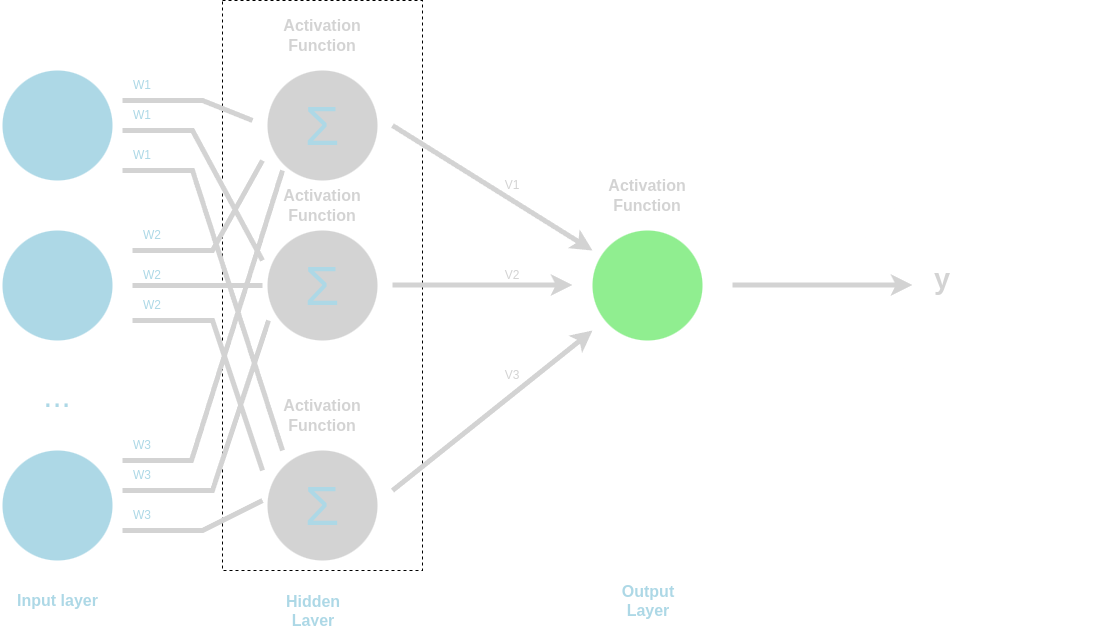
\includegraphics[width=\textwidth]{images/mlp.png}\caption{Multilayer Perceptron}\label{fig:mlp}
\end{figure}







\subsubsection{Domain Specific Language(DSL)}
It is a specialized language designed to address specific aspect or needs of a particular
language. Unlike general-purpose programming languages such as python, Java, or
C++ which are intended for a wide range of applications, \gls{dsl}s are optimized for a
particular set of tasks within a specific domain.We will be designing the simple lightweight Domain specific language to describe the
\gls{gui} . Elements in \gls{dsl} will be categorized into different
hierarchical structures on the basis of the position of the elements. Additionally to
reducing the size of the search space, the \gls{dsl} simplicity also reduces the size of the
vocabulary (i.e. the total number of tokens supported by the \gls{dsl}). To overcome this
problem, compact convolution transformers is introduced. This assists to avoid
overfitting and performs better than \gls{cnn} for small datasets. This model is flexible to
small model size and less parameter with achieving competitive results.

    \begin{figure}[H]
        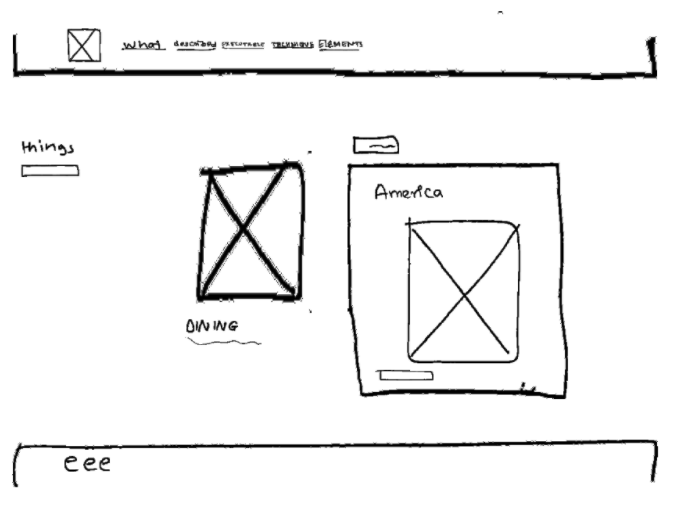
\includegraphics[scale=.6]{images/sample image.png}
        \caption{Sample Input Image}
        \label{fig:lsamp}
    \end{figure}




The sample \gls{dsl} for above image:

% Use the custom command to display the tree structure



\begin{verbatim}
    header{
        flex{
            logodiv{
                image
            }
            nav{
                navlink
                navlink
                navlink
                navlink
                navlink
            }
        }
    }
    container{[
        row{
            div-3{
                text-c
                input
            }
            div-3{
                image
                text
                paragraph
            }
            div-6{
                button
                card{
                    text-c
                    image
                    input
                }
            }
        }
    ]}
    footer{
        text
    }
    \end{verbatim}


\subsubsection{Customization}
Only transforming the sketch to HTML code is not enough. The sketch lacks colors,
and styling for various elements. It is merely a blue print for where each component are
located. The component must be styled accordingly for good look. This project will allow for some customizing by theme selection, color palate, font-selection, style
selection etc. The user can select appropriate style and designs as required.
The text content will be randomly generated text which the user can change. For image,
there is placeholder in which user can add link or choose from computer.
\subsubsection{Compiler}
Compiler is a computer program that translates computer code written in one
programming language into another language. In our context, Compiler will translate
the Domain Specific language that we designed into a HTML/CSS code. This compiler
will read a \gls{json} mapping file to define the conversion from \gls{dsl} tokens to HTML
tags. Then, it will systematically process the input, and build a hierarchical structure
that mirrors the nested elements of an HTML document.
It helps us to develop a flexible architecture that accommodates various output formats
beyond HTML, enabling cross-platform compatibility. Compiler can translate the
Domain Specific Language into suitable format for web, Android, and \gls{ios} platforms.
The compiler’s ability to target multiple platforms from a single \gls{dsl} source ensures
that application maintain consistent functionality and appearance across different
environments. \\
The web page is generated using compilation process that transforms custom made  
domain-specific language into fully functional web pages. The compiler operates
through a series of transformations, starting with a bare-bones \gls{dsl} specification 
that outlines the structural blueprint of the web page. This initial \gls{dsl} input from
the transformer intentionally omits specific content and styling details to maintain
flexibility and making training and testing process easier. The compilation process 
then add the data by incorporating user-defined content, images, links, and styling 
preferences through a \gls{dsl} mapping system that translates \gls{dsl} elements into a well-structured
\gls{json} representation . This \gls{json} intermediate format serves as a crucial waypoint, containing 
both structural 
information and dynamic content parameters from the user. In the final phase, the
 compiler transforms the \gls{json} into \gls{html} and \gls{css} files applying dynamic CSS variables
  for styling. This approach ensures that the final output remains both structurally 
  good and visually customizable, with the compiler bridging the gap between custom- 
  made DSL specifications and \gls{html} and \gls{css}.
\subsection{Activation Function}
Activation functions are mathematical equations that determine the output of a neural
network model. It can also be defined as transfer function. No matter how many hidden
layers are attached, every layer behaves the same way since the composite of two linear
functions is also a linear function. A non-linear activation function is required to learn
the difference between desired output and generated output. Thus the following
activation functions have been decided to be used.
\subsubsection{Softmax Function}
The Softmax function is sometimes called the soft argmax function, or multi-class
logistic regression since it is a generalization of logistic regression that can be used for
11 multi-class classification. The softmax function is ideally used in the output layer of the classifier where the probabilities are required to define the input images’ class. A
softmax function calculates the probabilities of each class which the input belongs. The
softmax units in the output layer always be equal to number of classes. The probability
distribution is different for different classes and the summation value of all probability
distribution is 1. The softmax function 4.4 provides the probability values for each
classes and class with highest probability value is consider as correct prediction.
\begin{equation}
\text{softmax}\sigma(\vec{z})_i = \frac{e^{z_i}}{\sum_{j} e^{z_j}}
\end{equation}
Where
\begin{align*}
    z_i &: \text{ elements of the input vector,} \\
    e^{z_i} &: \text{ standard exponential function applied to each element,} \\
    K &: \text{ number of classes in the multi-class classifier.}
\end{align*}\quad



The Softmax function is a function that turns a vector of K real values into a vector of
K real values that sum to 1. The input values can be positive, negative, zero, or greater
than one, but the values are converted to values between 0 and 1 by softmax. Thus now
they are interpreted as probability. Small or negative inputs are converted to a small
probability value.

\subsubsection{ReLU Function}
\gls{relu} is the most commonly used activation function in neural networks, whose
mathematical equation is: 

\begin{equation}
\text{ReLU}(x) = \max(0, x)
\end{equation}

So,if the input is negative, the output of ReLU is 0 and for positive values, it is x.

\begin{equation}
\frac{d}{dx} \text{ReLU}(x) = 
\begin{cases} 
0 & \text{if } x \leq 0 \\
1 & \text{if } x > 0
\end{cases}
\end{equation}

\begin{figure}[H]
    \centering
    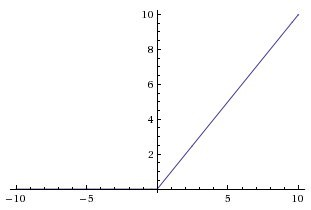
\includegraphics[scale=1]{images/RELU.jpg}
    \caption{Graphical Representation of ReLU Function}
    \label{fig:relu-}
\end{figure}



\subsection{Loss Function and Optimizer}
\subsubsection{Categorical cross entropy}
Categorical cross-entropy is a commonly used loss function in machine learning,
particularly in classification tasks where the model predicts the probability distribution
over multiple classes for each input sample. The loss is calculated by the following
formula:
\begin{equation}
\text{Loss} = -\sum_{i=1}^{Output size} y_i \log(\hat{y}_i)
\end{equation}
Where

\(\hat{y}_i\) = \(i\)th scalar scalar value in model output\\
\( y_i \)=Corresponding target value
output size = number of scalar values in the model output

\subsubsection{Adam Optimizer}
It is a popular optimization algorithm used in training neural network. It stands for
Adaptive Moment Estimation. It maintains two moving average vectors: the first
moment m (the mean) and the second moment v (the uncentered variance) of the
gradients. These moving average are used to adaptively adjust the learning rates for each parameters during training. Due to its simplicity of use, computational efficiency,
low memory requirements, and invariance to diagonal rescaling of the gradients, this
approach is well suited for scenarios involving high volumes of data and parameters.
\subsection{Performance Metrics}
\subsubsection{BLEU}
\gls{bleu} is an algorithm for evaluating the quality of
text which has been machine-translated from one natural language to another. This is
a common metric used in machine translation tasks, which seeks to measure how
closely a machine-generated text resembles what a human would have generated, given
the same input. It is based on n-gram based precision. Four sub metrics are denotes as
BLEUn, for n = 1, 2, 3, 4. For a candidate sentence a and a set of reference sentences
b, the BLEU score is calculated as:
\begin{equation}
\text{BLEU}_n(a, b) = \frac{\sum_{w_n \in a} \min\left(\text{count}_a(w_n), \max_{j=1, \ldots, |b|} \text{count}_{b_j}(w_n)\right)}{\sum_{w_n \in a} \text{count}_a(w_n)}
\end{equation}
where wn denotes n-gram, counta(wn) denotes count of n-gram wn in sentence
\subsubsection{ROUGE}
ROUGE (Recall-Oriented Understudy for Gisting Evaluation) is an evaluation metric
specially designed for automatic summarization that can be used for machine
translation. It measures the overlap of n-grams between the generated sequence and
reference sequence. The ROUGE score is calculated as:
\begin{equation}
\text{ROUGE-N Precision} = \frac{\sum_{n}\text{count}_{\text{match}}(n)}{\sum_{n}\text{count}_{\text{generated}}(n)}
\end{equation}
\begin{equation}
\text{ROUGE-N Recall} = \frac{\sum_{n}\text{count}_{\text{match}}(n)}{\sum_{n}\text{count}_{\text{reference}}(n)}
\end{equation}
\begin{equation}
\text{ROUGE-N F1} = \frac{2 \times \text{ROUGE-N Precision} \times \text{ROUGE-N Recall}}{\text{ROUGE-N Precision} + \text{ROUGE-N Recall}}
\end{equation}





\subsection{Flowchart}
\subsubsection{During Training}
\begin{figure}[H]
    \centering
    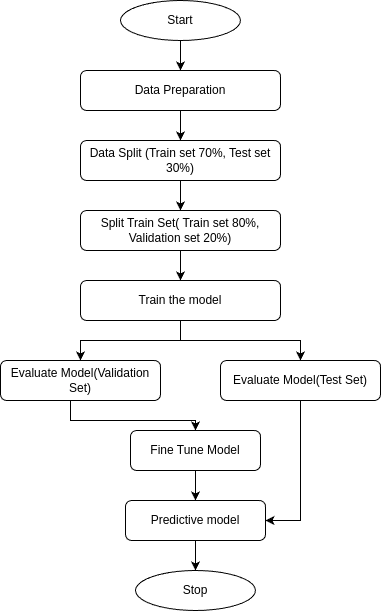
\includegraphics[scale=0.8]{images/training flowchart.png}
    \caption{Training Flowchart}
    \label{fig:flowtra}
\end{figure}

\subsubsection{During Testing}
 \begin{figure}[H]
 \centering
        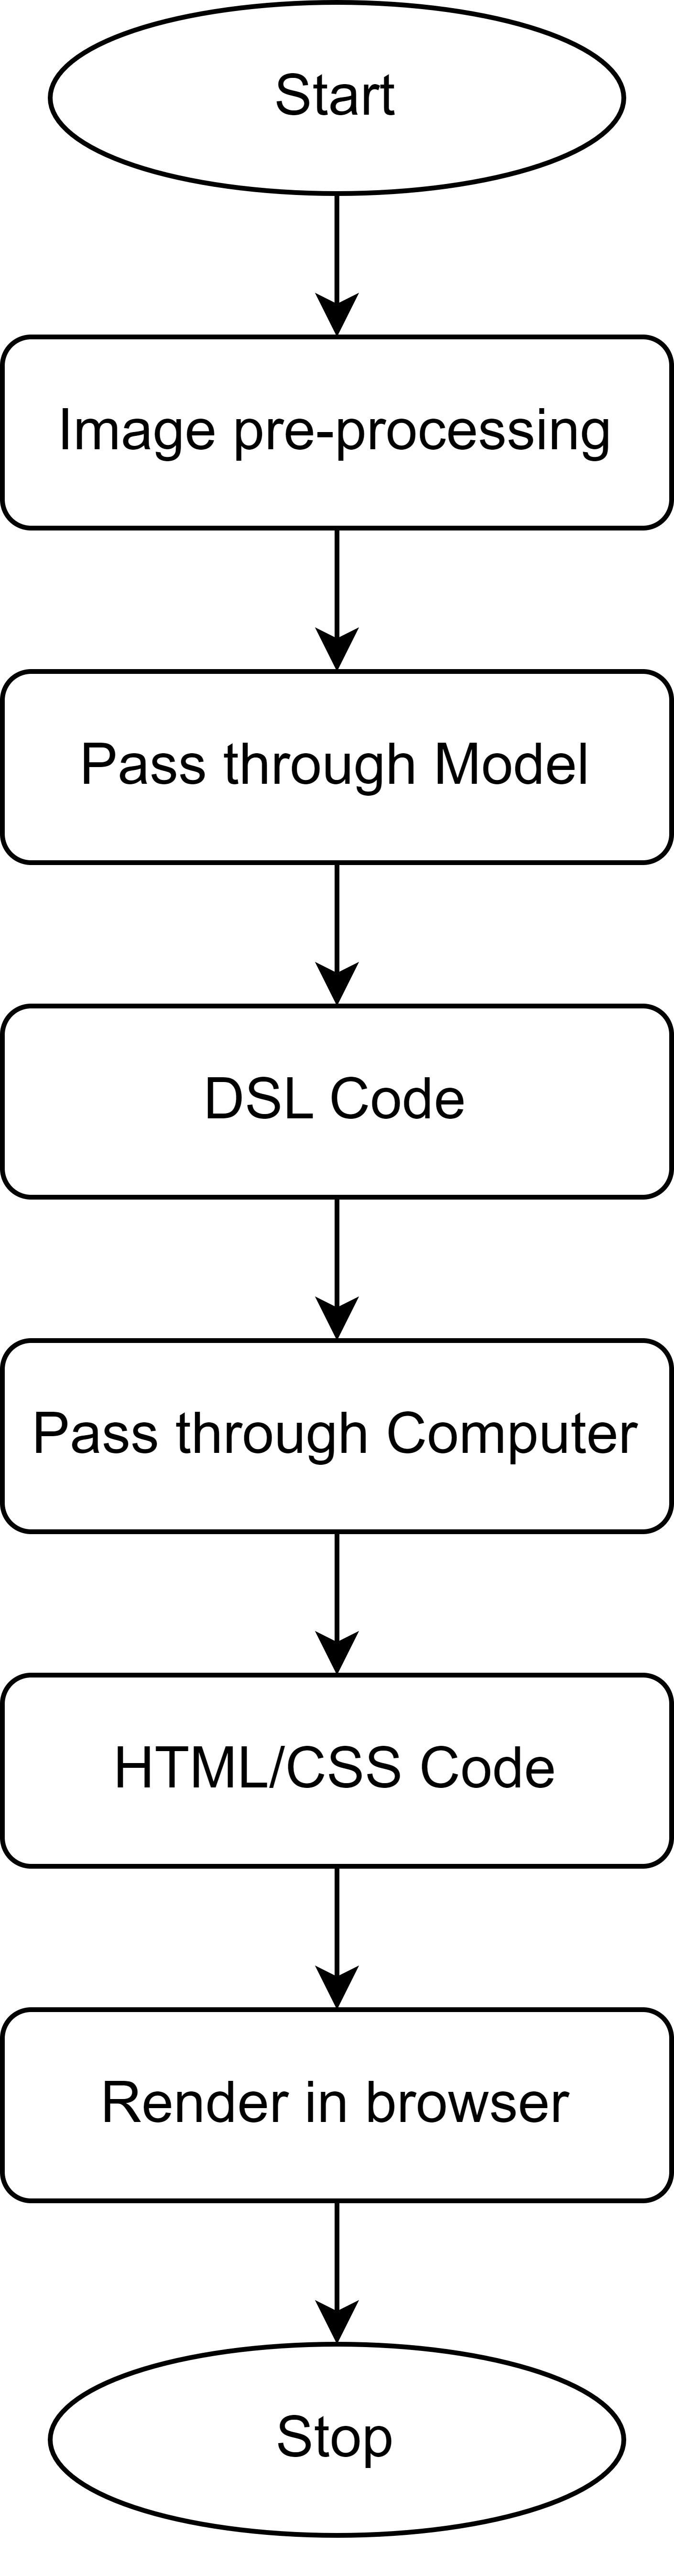
\includegraphics[scale=1.5]{images/testing flowchart.png}
        \caption{Testing Flowchart}
        \label{fig:flowtr}
    \end{figure}


    \pagebreak

\section{\MakeUppercase{Implementation Details}}
\subsection{Dataset Generator Implementation}
Initially, we collected the multiple number of hand-drawn sketches for the each element
under consideration. These sketches is combined to generate any number of data as
required.
\subsubsection{Steps taken in Dataset Generation}
\textbf{Random \gls{dsl} generator}\\
First we have to generate a \gls{dsl} code which is created by using the custom made rule
which is described below. Different \gls{dsl} code is generated by mixing the different
possible combination of the element.\\
\textbf{Compiling the \gls{dsl} Code}\\
After generating the \gls{dsl} Code, we compiled or mapped the produced \gls{dsl} code to
proper HTML code.\\
\textbf{Rendering the produced HTML Code}\\
We then rendered the \gls{html} code in chrome browser and also use the special \gls{css} file
during rendering. Different elements are rendered with specified background color. The
javascript file is also used to dynamically set random height, width and position for
each element. Then, screenshot is taken of the rendered page.\\
\textbf{Finding the outline of the different element}\\
For detecting each element, we filter the background color of each element and by using
contour detection obtain the dimensions and position of the specific element.
\textbf{Placement of hand-drawn sketch}\\
The aspect ratio of the hand drawn sketches is compared with the aspect ratio of the
bounding box for each element. The sketches are sorted according to the best match
aspect ratio. The random sketch among top 8 sketches is placed in the location. \\
\textbf{Rules for creating \gls{dsl}}\\
We have defined the structure and rules for generating random website layouts in a
\gls{dsl}. We established a hierarchical structure of webpage
elements, where each key represents a component and its value lists possible child
components. For instance, the 'root' element can contain 'header', 'container', and
'footer', while a 'row' can have various sizes of div elements. We also defined different
ways to divide a row into columns, based on a 12-column grid system which common
in responsive web design. There is also constraints and behaviors for different elements,
such as the minimum and maximum number of occurrences, whether children should
be generated in a specific order, and how to apply the division combinations for rows.
This structure allows for the generation of diverse yet constrained layouts and also
ensuring essential elements are present, allowing for variable numbers of containers
and rows, providing flexibility in column divisions, and setting limits on the number of
elements within components.
\subsection{Model Implementation}
We have designed a transformer-based architecture to convert the sketch images into
the \gls{dsl} code. It consists of an encoder that processes input images (sketches) and a
decoder which generates the corresponding code. Our model combines \gls{cnn} for image processing with transformer layers for sequence
modeling, which makes it well-suited for translating visual information in images into
textual output, which is \gls{dsl} code.
\subsubsection{Input Processing}
The model takes two inputs: an image input with shape (None, 850, 600, 1),
representing grayscale sketches, and a text input with shape (None, 120), representing
the \gls{dsl} code associated with the input sketch image.
\subsubsection{Convolutional Tokenizer}
The first major component in our model is the Convolutional Tokenizer. This custom
layer processes the input image through a series of convolutional and pooling
operations, converting the 2D image into a sequence of feature vectors. Output shape of this component is (None, 513, 128) which means it transformed the image into 513
tokens, each with 128 dimensions.\\
\textbf{Convolutional Layers}\\
The tokenizer uses a series of convolutional layers (Conv2D) with increasing numbers
of filters (32, 64, 64, 128, 128). Each convolutional layer is followed by zero-padding
and max-pooling operations. This structure helps in reducing the spatial dimensions of
the image while increasing the depth, which is number of channels. Max-pooling layers
are used after each convolution to reduce the spatial dimensions. This helps in capturing
hierarchical features and reducing computational complexity. Dropout layers are
inserted twice in the network after the second and fourth convolutional blocks to
prevent overfitting.The layers are as follows:
\begin{enumerate}
    \item First convolutional layer: It contains 32 filters of kernel size of 7x7 with stride of 1
with no padding and have ReLU activation function. Then, ZeroPadding2D adds a
padding of 1 around the feature map to preserve spatial dimensions. Then, the maxpooling layer of 3x3 pooling window and stride of 2 is added.
\item  Second convolutional layer: It contains 64 filters of kernel size of 5x5 with stride of
1 with no padding and have ReLU activation function. Then, ZeroPadding2D adds a
padding of 1 around the feature map. Then, the max-pooling layer of 3x3 pooling
window and stride of 2 is added. And, dropout is applied with a rate of 0.1 to prevent
overfitting.
\item Third convolutional layer: It contains 64 filters of kernel size of 3x3 with stride of 1
with no padding and have ReLU activation function. Then, ZeroPadding2D adds a
padding of 1 around the feature map. Then, the max-pooling layer of 3x3 pooling
window and stride of 2 is added
\item  Fourth convolutional layer: It contains 128 filters of kernel size of 3x3 with stride of
1 with no padding and have ReLU activation function. Then, ZeroPadding2D adds a
padding of 1 around the feature map. Then, the max-pooling layer of 3x3 pooling
window and stride of 2 is added. And, dropout is applied with a rate of 0.1.
\item . Fifth convolutional layer: It contains 128 filters of kernel size of 3x3 with stride of 1
with no padding and have ReLU activation function. Then, ZeroPadding2D adds a
padding of 1 around the feature map. Then, the max-pooling layer of 3x3 pooling
window and stride of 2 is added. 


\end{enumerate}
Then the output from the convolutional tokenizer is flatten to shape of (513,128).
\subsubsection{Positional Embedding}
After the convolutional tokenization, positional encoding is added to the token
embeddings. We have used the sinusoidal Positional Encoding. This is crucial for the
transformer architecture to understand the spatial relationships between different parts
of the image. Then we combine the tokenized images features with positional
information.
\subsubsection{Encoder}
The encoder consists of three transformer blocks. Each block includes 
layer normalization, multi-head attention (self-attention), residual connection,
feed-forward neural network, and another residual connection. The encoder processes
 the image tokens (513x128) to create a rich representation for the decoder. The output of each
encoder block maintains the 513x128 dimension.\\
\textbf{Layer normalization}\\
Each layer normalization has 256 parameters and normalizes the inputs across the 128
feature dimensions to improve training stability.\\
\textbf{Multi-head attention(Self-attention)}\\
Each multi-head attention layer has 329,728 parameters. We have use 5 number of
heads. The input and output dimensions are both 513x128.\\
\textbf{Residual Connection}\\
Residual connections add the input (513x128) to the output of the attention layer.\\
\textbf{Feed-forward Neural Network}\\
It consist of two dense layers. The first dense layer of size 513x128 which consist of
16,512 parameters. Then, dropout layer is added. After that, second dense layer of same
size with same number of parameters are added. Then, another dropout is added.
\subsubsection{Decoder}
The decoder is more complex, consisting of four transformer blocks. It takes the
embedding of the input sequence (120x128) and processes it while attending to the
encoder's output (513x128).
Each block in the decoder includes:\\
\textbf{Self-attention Layer}\\
This layer has 329,728 numbers of parameters with input and output dimension of
120x128. This layer mask the future token ensuring that the prediction for a given token
is done only using previous tokens.\\
\textbf{Cross-attention Layer}\\
It has 329,728 numbers of parameters and attends to the encoder output (513x128)
while processing the 120x128 decoder sequence.\\
\textbf{Feed-forward Network}\\
It consist of two dense layer of size 120x128 consisting 16,512 numbers of parameters
and each dense layer is followed by the dropout layer.\\
\textbf{Layer Normalization and Residual Connections}\\
Each layer normalization has 256 parameters, normalizing across the 128 feature
dimensions. Residual connections add the input (120x128) to the output of each sublayer.
\subsubsection{Attention Mechanism}
The model uses several multi-head attention layers. In the encoder, these are selfattention layers, allowing each token to attend to all other tokens in the image
representation. In the decoder, there are both self-attention layers for processing the
output sequence and cross-attention layers for attending to the encoder's output.
\subsubsection{Masking}
The model implements causal masking in the decoder's self-attention layers. It ensures
that each position in the output sequence can only attend to previous positions which is
crucial for autoregressive generation.
\subsubsection{Output Layer}
The final layer is a dense layer with 31 units, corresponding to the vocabulary size of
the output tokens (minus one, accounting for a start token). This layer produces the
logits for each token in the vocabulary at each position in the output sequence.
\subsection{Model Complexity}
The model has a total of 3,488,447 trainable parameters, which is relatively compact
for a task of this complexity. This model have a balance between model capacity and
computational efficiency.
\subsection{Vocabulary of Model}
The \gls{dsl} used in this project consists of total 32 different symbols and words. \texttt{<Start>},
\texttt{<End>} and \texttt{<Pad>} are special symbols. The textual representation is converted to vector
form. For each words or symbols, unique number from 0 to 31 is assigned. \texttt{<Pad>}
symbol is assigned 0 which is added to make input uniform. \texttt{<Start>} symbol is assigned
31. These vector information is passed as the input to model. The embedding layer
converts one dimensional vector to vector of size corresponding to projection
dimensions.
\subsection{Output \gls{dsl}}
Our transformer model gives DSL as an output which only denotes the elements present in the given 
web page. The content required to effectively complete the element such as text, image and \gls{url} 
links are not present in the generated DSL code, which we have to add after. This conversion have 
the several steps which is given in the following points. 
\subsection{User Interface}
User can change the style of the page from the interface. Text, image, link, color, font size, 
spacing can be change using the interface. Change message are passed to the compiler in the \gls{json} format. 
\subsection{\gls{dsl} to \gls{json} compiler}
First, we convert the generated \gls{dsl} output into the \gls{json} format by adding relevant information into it.
Text, image, \gls{url} are added in this process which is obtained from the user through the User Interface. It is converted
using the DSL mapping file which contains all the information related to the DSL element. Generated \gls{json} file 
can be used to generate the required HTML and CSS. JSON also contains the style required to customize the color based
 on the user input. All the data required for the webpage is passed through the \gls{json} file.
\subsection{\gls{json} to \gls{html} compiler}
\gls{json} file obtained from the \gls{json} compiler consist all the information required to convert it into the required 
HTML and CSS file. Each \gls{json} file is mapped according to the DSL mapping file and according to the hierarchy of the 
element, it is render to get HTML file. CSS file is created using the dynamic \gls{css} variable which helps in inserting 
the requirement of the user from the \gls{json} file. We, then get the required html file with its corresponding style in the CSS file.

\begin{figure}[H]
    \centering
           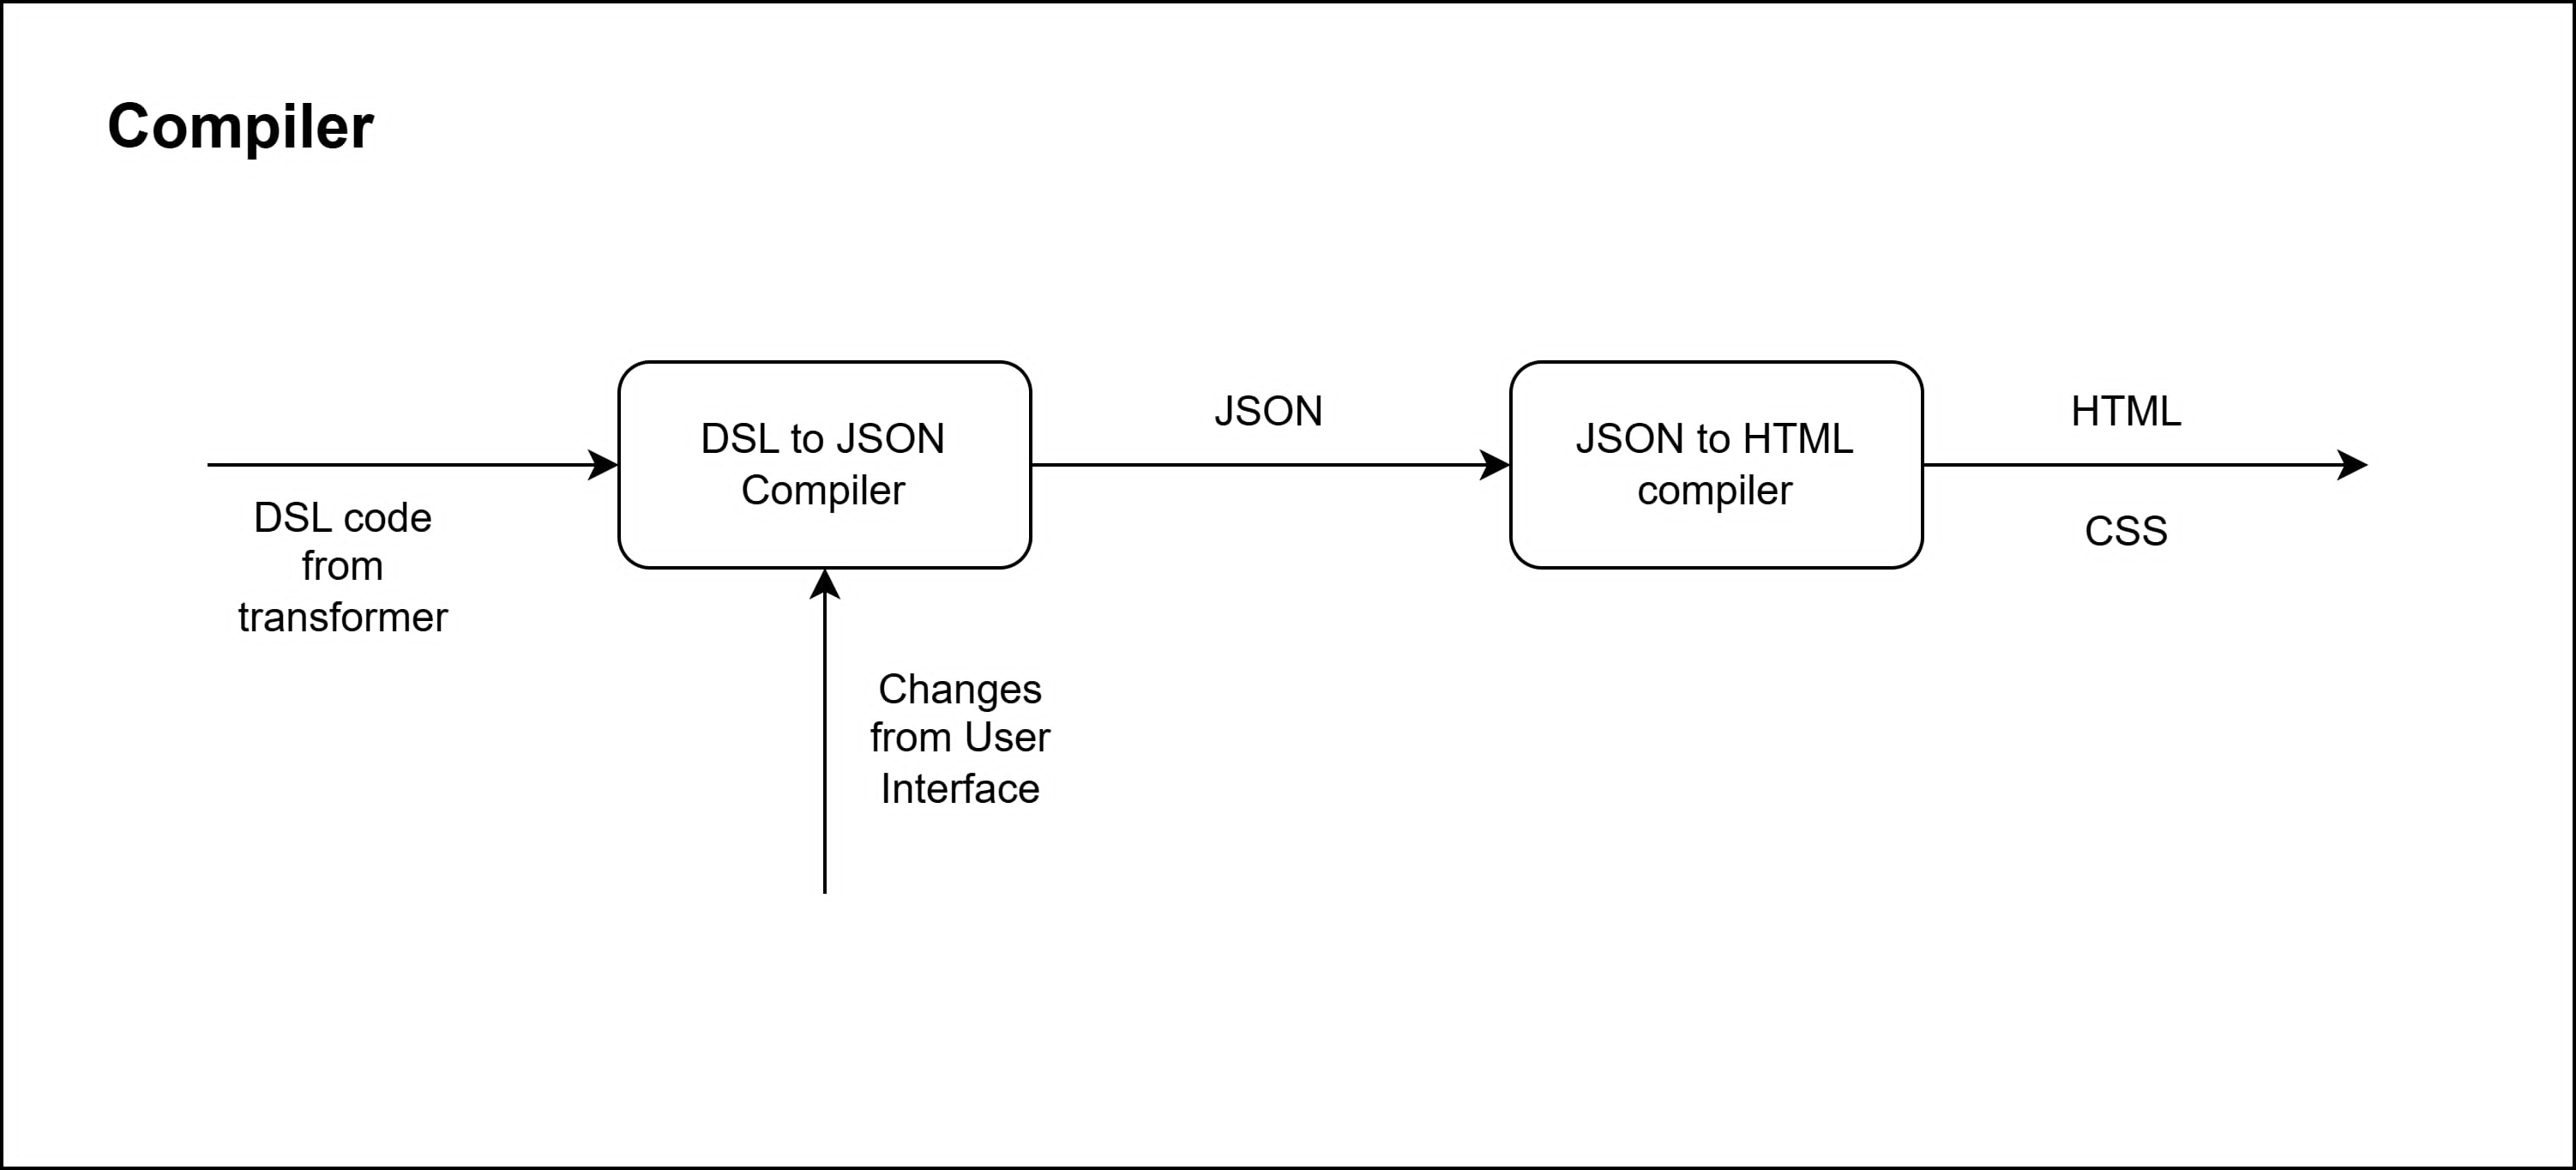
\includegraphics[scale=0.15, trim=100 200 200 0]{images/compiler flow.jpeg}
           \caption{Compiler Flow}
           \label{fig:Compflow}
       \end{figure}
   
 \subsection{Training Details}
The model is trained on paired sketch-code data using supervised learning. It employs
teacher forcing by feeding ground truth tokens to the decoder during training. The
objective is to minimize cross-entropy loss between predicted and actual tokens. Endto-end training optimizes both convolutional and transformer layers. Data augmentation
is used to improve training stability and model generalization.
\subsection{Testing Details}
During testing, the model generates code iteratively, one token at a time. It processes
the input sketch and predicts tokens sequentially, using previously generated tokens as
input for subsequent predictions. Performance is evaluated using metrics like \gls{bleu}
and \gls{rouge} score. Human evaluation is also necessary to assess the generated code's
quality and input image quality.
\pagebreak
\section{\MakeUppercase{Result and Analysis}}





\subsection{Model Training}
The model is trained for 8 epochs taking batch size of 32. The training set consists of
8951 samples and testing set consists of 2238 samples. All these samples are generated
using random dataset generator.

\subsubsection{Loss vs Epoch Graph}
 \begin{figure}[H]
        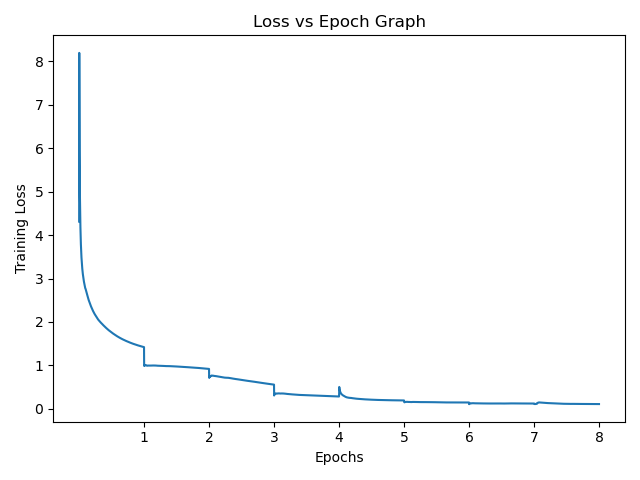
\includegraphics[scale=1]{images/Training Loss.png}
        \caption{Loss vs Epoch graph for training time}
        \label{fig:lvsepocht}
    \end{figure}
     \begin{figure}[H]
        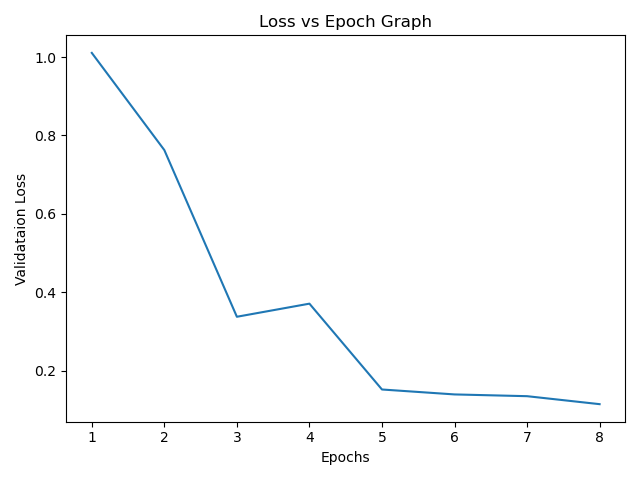
\includegraphics[scale=.8]{images/Validataion Loss.png}
        \caption{Loss vs Epoch graph for validation time}
        \label{fig:lvsepochv}
    \end{figure}


        
        Initially, the loss for the model is very high. In first epoch, the loss gradually decreased
and reached around 1.5. In the following epochs, the loss decreased steadily and
reached to 0.1 in the final epoch. The loss in validation set also remain comparable to
that of training set throughout the training which confirms model didn’t over fit for the
training data.
        \subsubsection{Evaluation}
        After training for 8 epochs, the model is evaluated on the test data. The BLEU and
ROUGE evaluation metrics are used to evaluate the model.\\
\textbf{BLEU Score}\\
The average BLEU score for n-grams 1, 2, 5 and 10 is as follows:
\begin{itemize}
    \item 1-grams BLEU Score: 0.9544114683715649
\item 2-grams BLEU Score: 0.9378854888760932
\item 5-grams BLEU Score: 0.8867411989388778
\item 10-grams BLEU Score: 0.7982317463855622
\end{itemize}
The above observation shows that the model performed well for the given testing data.
The average BLEU-1 score of 0.95 indicate that the generated \gls{dsl} closely match the
reference \gls{dsl}. The BLEU score decreased for increasing n grams but the score is still
good which indicates model is good predicting short sequences. The BLEU-10 score is
also good (0.79). So, it also predicted longer sequence.
The individual BLEU-10 score in sorted order is plotted in the graph. It can be seen that
the score is higher than 0.6 for most of the samples. There are plenty of samples with
bleu scores above 0.9. So, the model performed well for the testing data.
 \begin{figure}[H]
        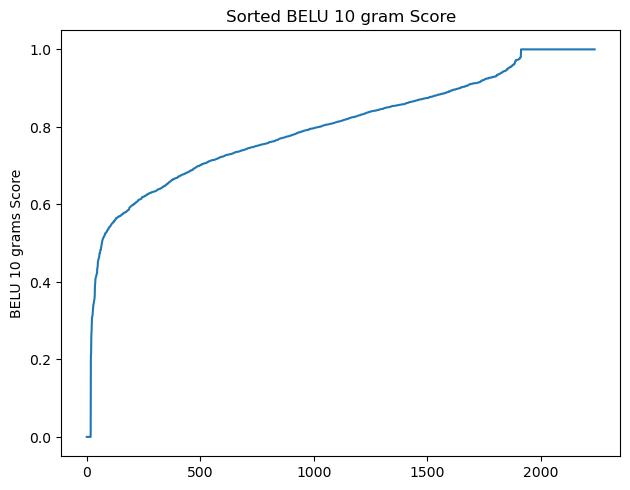
\includegraphics[scale=.8]{images/bleu in sorted order.png}
        \caption{BLEU-10 Scores in sorted order}
        \label{fig:bleu10}
    \end{figure}


    
        
\textbf{ROUGE Score}\\
The average ROUGE Scores are tabulated below:
    Inserting table:
    \begin{table}[H]
        \caption{ROUGE Scores for test data}
        \label{tab:sample}
        \centering
        \begin{tabular}{|c|c|c|c|}
            \hline
            \textbf{Metric} & \textbf{Precision} & \textbf{Recall} &\textbf{F1-Score}\\
            \hline
            ROUGE-1 & 0.9481 & 0.9486 &0.9652 \\
            \hline
            ROUGE-5 & 0.7806&0.8112 & 0.7948 \\
            \hline
            ROUGE-L & 0.9428 & 0.9791 & 0.9598 \\
            \hline
        \end{tabular}
    \end{table}
    From above table, ROUGE-1 has high F1-score of 0.96. This indicates the predicted
tokens matches 96\% with the reference tokens. The ROUGE-5 F1-score is 0.79. It has
decreased drastically but it is still a good score. The high recall of 0.97 for ROUGE-L
indicates that the generated \gls{dsl} captures most of the longest common subsequences
from the reference. This indicates the generator maintains correct sequence and structure of \gls{dsl}. The graph below shows that the F1-score for almost all samples is
above 0.9 which is good performance.

 \begin{figure}[H]
        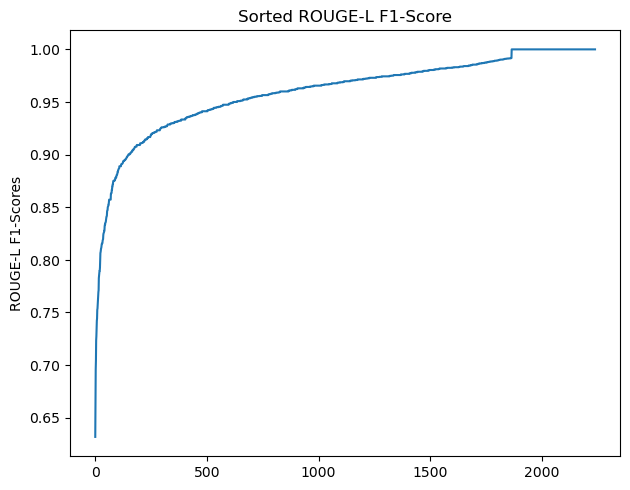
\includegraphics[scale=.8]{images/rouge-L F1-scores in sorted order.png}
        \caption{ROUGE-L F1-Scores in sorted order}
        \label{fig:rouge-l-F1 score}
    \end{figure}






\subsection{Customization}
User can style and customize the layout and visuals of the generated webpage.
\subsubsection{\gls{ui}}
Here, is the screenshot of the interface which can be used to change the style of the 
generated web page. First, they have to upload the image and then, they can customize the webpage. Here, user can save the desired webpage and they will get html, CSS for that page.



\begin{figure}[H]
    \centering
           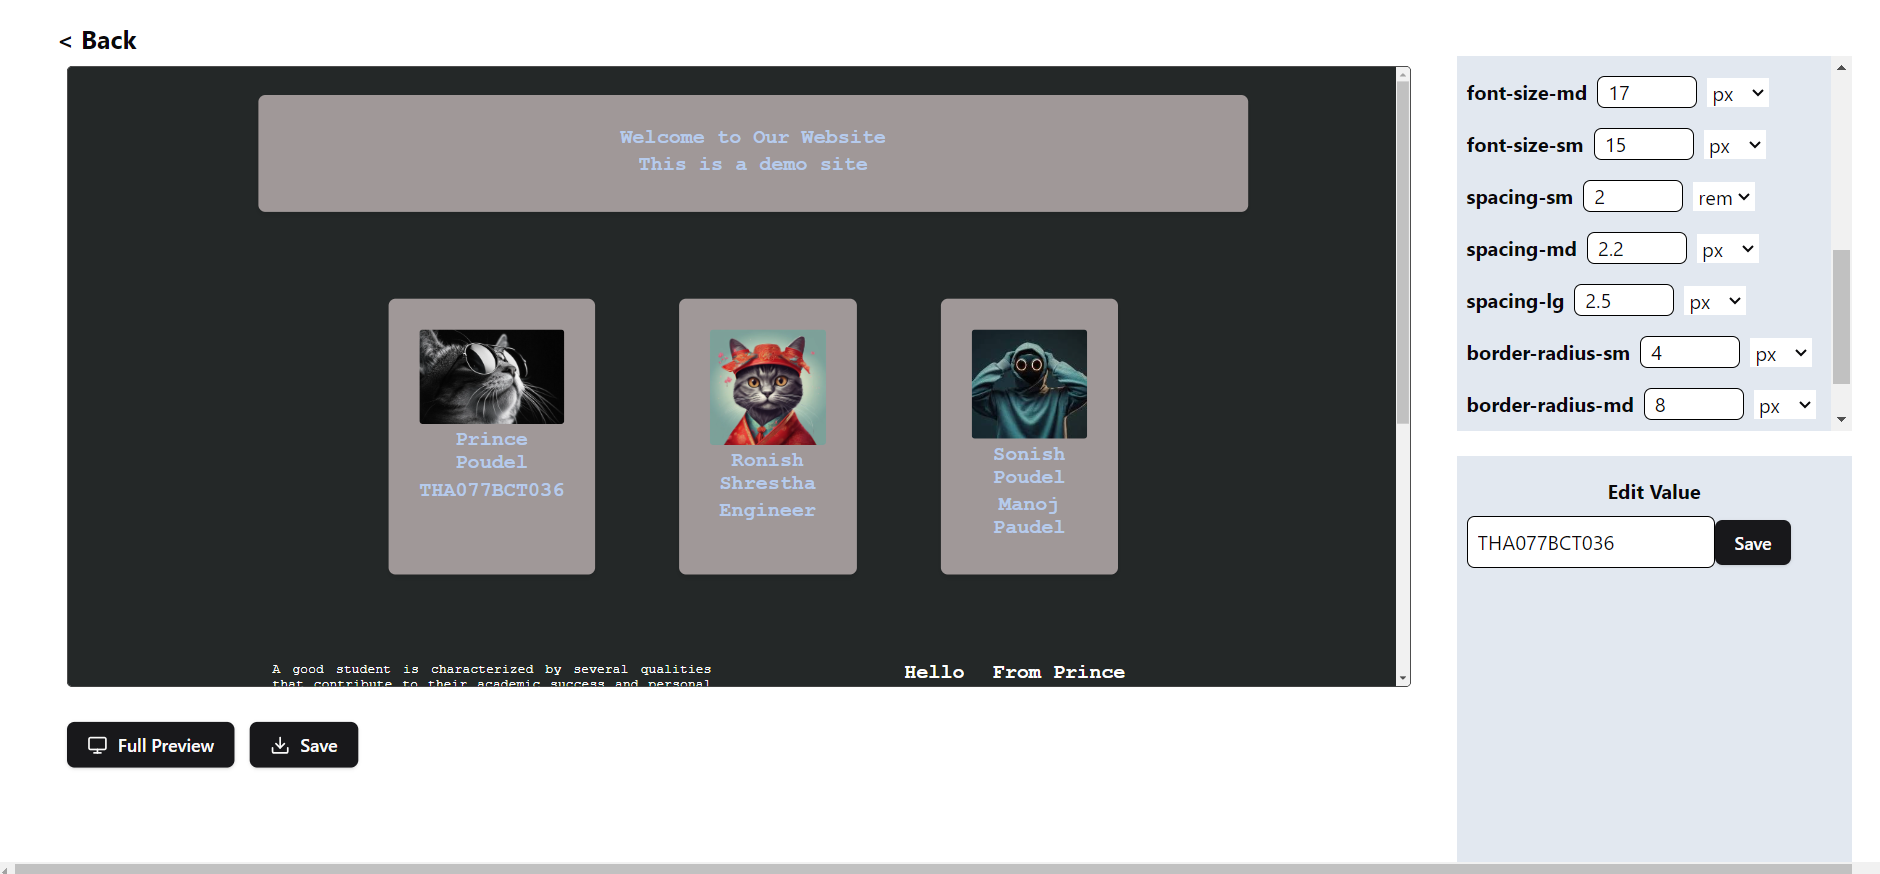
\includegraphics[scale=0.25, trim=230 10 190 10]{images/user interface.png}
           \caption{User Interface}
           \label{fig:ui}
       \end{figure}
   

\subsubsection{Full Webpage}
This is the webpage that a user can get after customization.

\begin{figure}[H]
    \centering
           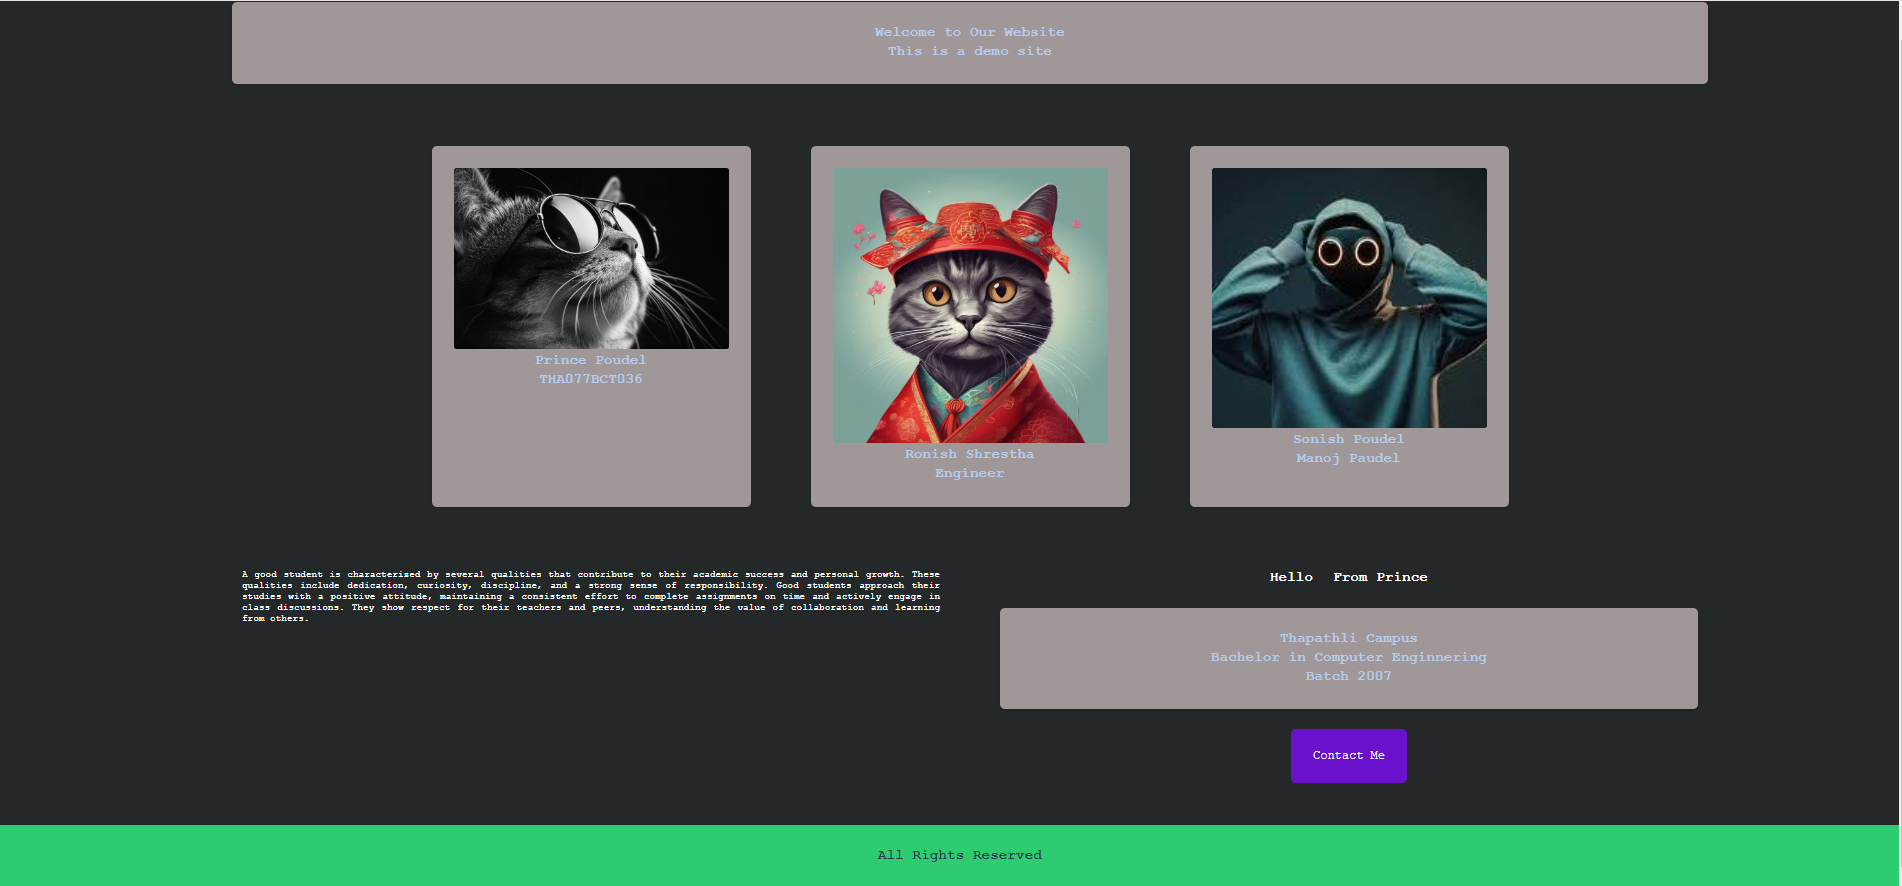
\includegraphics[scale=0.25,trim=230 10 190 10, clip]{images/full webpage.png}
           \caption{Full webpage}
           \label{fig:fullweb}
       \end{figure}


\subsubsection{Customization Options}
Different customization options are available to change the style of webpage. Mainly, user can change the color, text,  
size and text font.  All the options available are given below.

\begin{figure}[H]
    \centering
    \begin{minipage}{0.5\textwidth} % Adjust width to ensure spacing
        \centering
        \vspace{+64pt}
        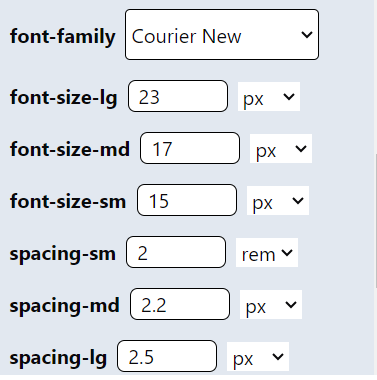
\includegraphics[width=\linewidth]{images/customization 1.png}
        \caption{Font Customization}
        \label{fig:c1}
    \end{minipage}%
    \hfill
    \begin{minipage}{0.5\textwidth}
        \centering
        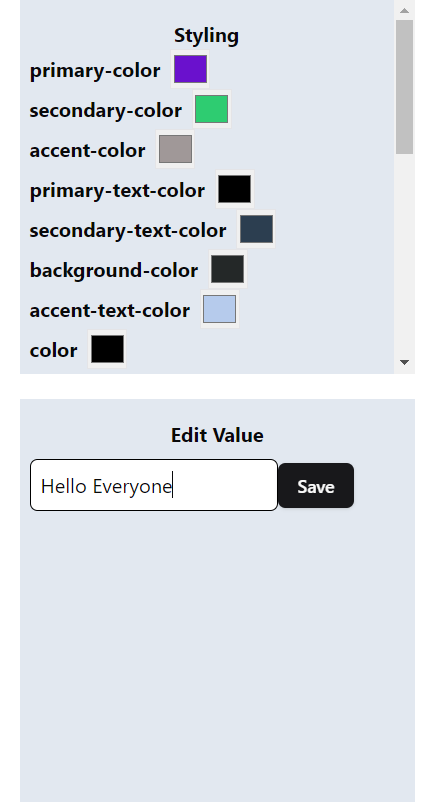
\includegraphics[width=\linewidth, trim=0 250 0 0, clip]{images/customization 2.png}
        \caption{Color Customization}
        \label{fig:c2}
    \end{minipage}
\end{figure}


\subsubsection{\gls{json} file}
This is the sample of the JSON file which have information about the element and the styles. It also carries the changes 
specified by the user through the User interface. Node key helps in carrying the information about the hierarchical structure of the webpage.
 
\begin{verbatim}
    {
        "node": {
          "element": "root",
          "nodes": [
            {
              "element": "header",
              "nodes": [
                {
                  "element": "flex",
                  "nodes": [
                    {
                      "element": "logodiv",
                      "nodes": [
                        {
                          "element": "image",
                          "nodes": [],
                        }
                      ]
                    }
                  ]
                }
              ]
            },
            {
              "element": "container",
              "nodes": [
                {
                  "element": "row",
                  "nodes": [
                    {
                      "element": "div-6",
                      "nodes": [
                        {
                          "element": "image",
                          "nodes": [],
                          "url": "https://..........."
                        }
                      ]
                    }
                  ]
                },
                {
                  "element": "row",
                  "nodes": [
                    {
                      "element": "div-12",
                      "nodes": [
                        {
                          "element": "text",
                          "nodes": [],
                          "text": "About Us"
                        },
                        {
                          "element": "paragraph",
                          "nodes": [],
                          "text": "We …………”
                        }
                      ]
                    }
                  ]
                }
              ]
            }
          ],
          "styles": {
            "accent-color": "#e74c3c",
            "accent-text-color": "black",
            "background-color": "#ecf0f1",
            "border-radius-lg": "12px",
            "border-radius-md": "8px",
            "border-radius-sm": "4px",
            "color": "#1c1717",
            "font-family": "Arial",
            "font-size-lg": "25px",
            "font-size-md": "16px",
            "font-size-sm": "18px",
            "primary-color": "#6a11cd",
            "primary-text-color": "white",
            "secondary-color": "#2ecc71",
            "secondary-text-color": "#2c3e50",
            "spacing-lg": "2rem",
            "spacing-md": "1.5rem",
            "spacing-sm": "1rem"
          }
        }}

\end{verbatim}



\subsubsection{Html File}
This is the sample of the HTML and CSS file which is compiled from the JSON. 
\begin{verbatim}
    <head>
    <meta charset="UTF-8" />
    <meta name="viewport" content="width=device-width, initial-scale=1.0" />
    <title>Generated Page</title>
  </head>
  <body>
    <div id="root" class="root" data-id="110">
      <header class="header" data-id="111">
        <div class="flex" data-id="112">
          <div class="logodiv" data-id="113">
            <img
              src="https://..."
              class="image"
              data-id="114"
            />
          </div>
        </div>
      </header>

      <div class="container" data-id="115">
        <div class="row" data-id="116">
          <div class="div-6" data-id="117">
            <img
              src="https://....
              class="image"
              data-id="118"
            />
          </div>
        </div>
        <div class="row" data-id="119">
          <div class="div-12" data-id="120">
            <div class="text" data-id="121">About Us</div>
            <p class="paragraph" data-id="122">We are</p>
          </div>
        </div>
      </div>
    </div>
  </body>
  
</html>

\end{verbatim}

    \subsection{Sample Generated Datasets}
\textbf{Sample 1}
\begin{verbatim}
    container {
        row {
            div-6 {
                image
                paragraph
            }
            div-6 {
                flex-r {
                    button
                    button
                    text
                }
                carousel
                button
            }
        }
        row {
            div-9 {
                carousel
                input
                text
            }
            div-3 {
                card {
                    image
                    paragraph
                    text-c
                }
                paragraph
            }
        }
        row {
            div-3 {
                card {
                    input
                    input
                }
                input
            }
            div-3 {
                card {
                    paragraph
                    text-c
                }
                button-c
            }
            div-6 {
                paragraph
                button
                text
            }
        }
    }
    footer {
        text-c
    }
    \end{verbatim}
    

\begin{figure}[H]
    \centering
    \begin{minipage}{0.35\textwidth}
        \centering
        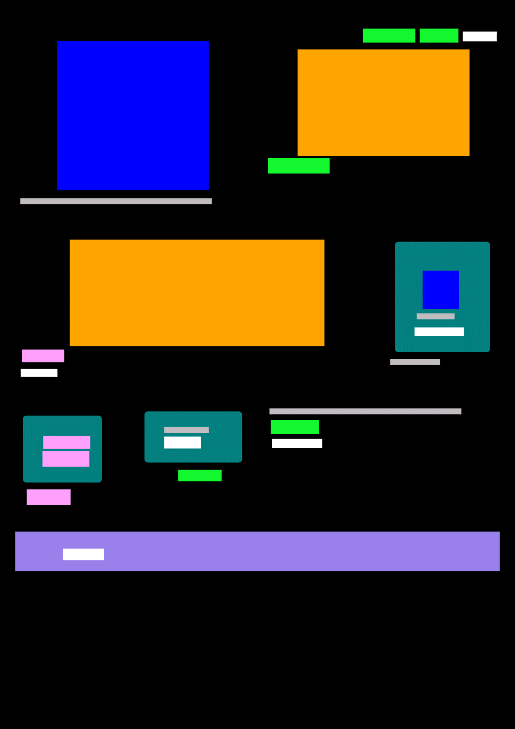
\includegraphics[width=\linewidth]{images/sample1-rendered.png}
        \caption{Rendered HTML}        
        \label{fig:s1}
    \end{minipage}\hfill
    \begin{minipage}{0.35\textwidth}
        \centering
        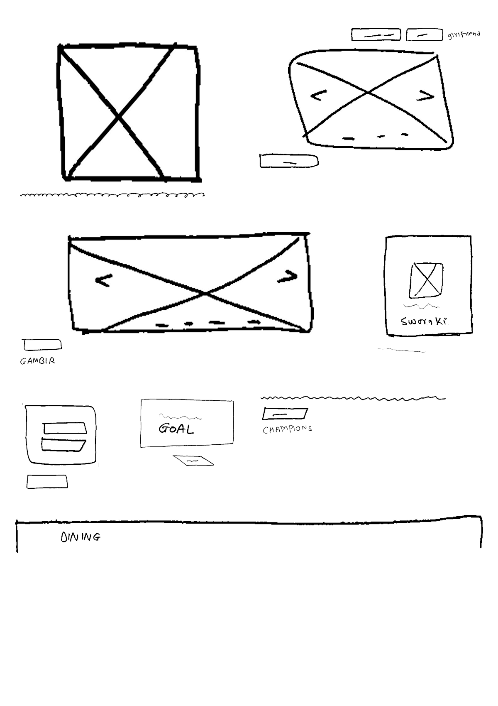
\includegraphics[width=\linewidth]{images/sample1-sketch.png}
        \caption{Sketch}
        \label{fig:s2}
    \end{minipage}
\end{figure}
\vspace{1em} 

    
\textbf{Sample 2}
\begin{verbatim}
    header {
        flex-sb {
            logodiv {
                image
                text
            }
            nav {
                navlink
                navlink
                navlink
                navlink
            }
        }
    }
    container {
        row {
            div-9 {
                input
                flex-sb {
                    button
                    button
                    button
                    text
                }
                table
                button
            }
            div-3 {
                card {
                    paragraph
                    text-c
                    paragraph
                }
                paragraph
            }
        }
        row {
            div-3 {
                button-c
                text
                image
                input
            }
            div-6 {
                paragraph
                carousel
                paragraph
            }
            div-3 {
                text
                button
                image
            }
        }
        row {
            div-3 {
                text-c
                card {
                    button
                    image
                }
                input
            }
        }
    }
    \end{verbatim}    
    \begin{figure}[H]
    \centering
    \begin{minipage}{0.35\textwidth}
        \centering
        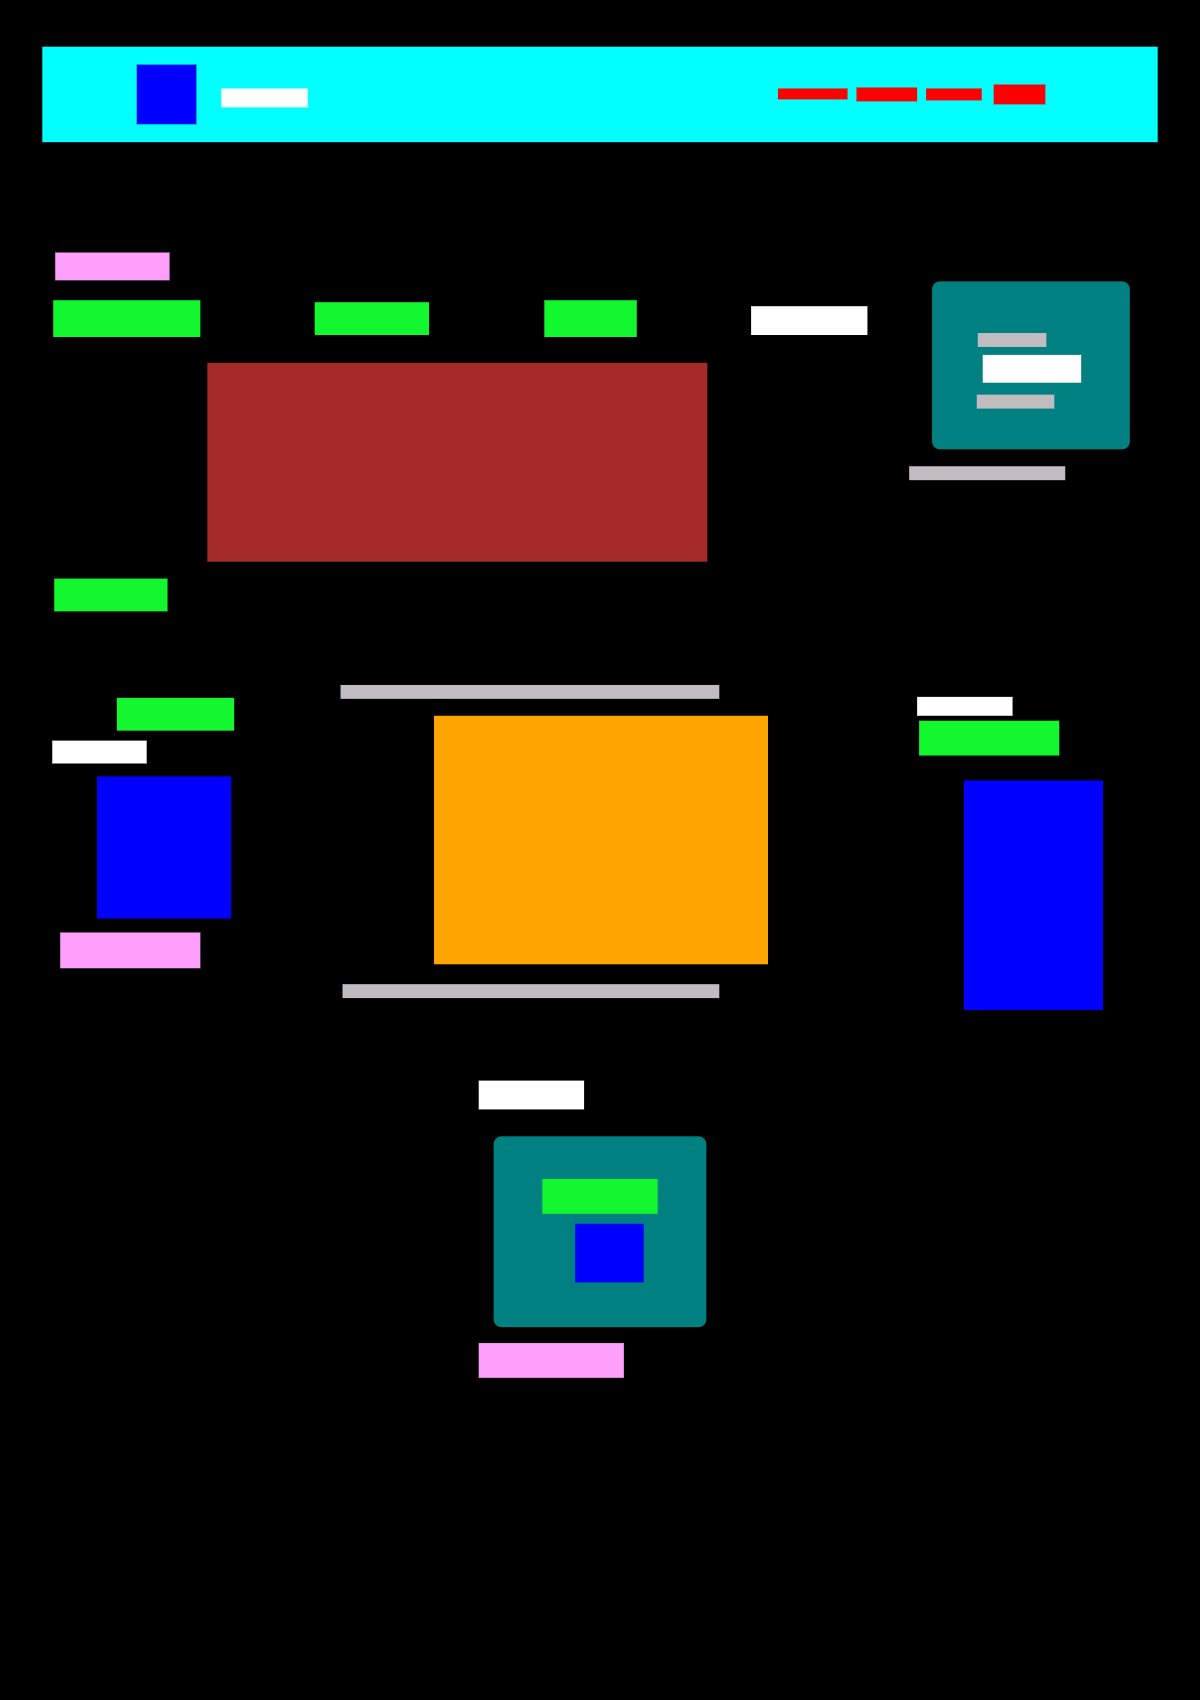
\includegraphics[width=\linewidth]{images/sample2-rendered.png}
        \caption{Rendered HTML}
        \label{fig:s21}
    \end{minipage}\hfill
    \begin{minipage}{0.35\textwidth}
        \centering
        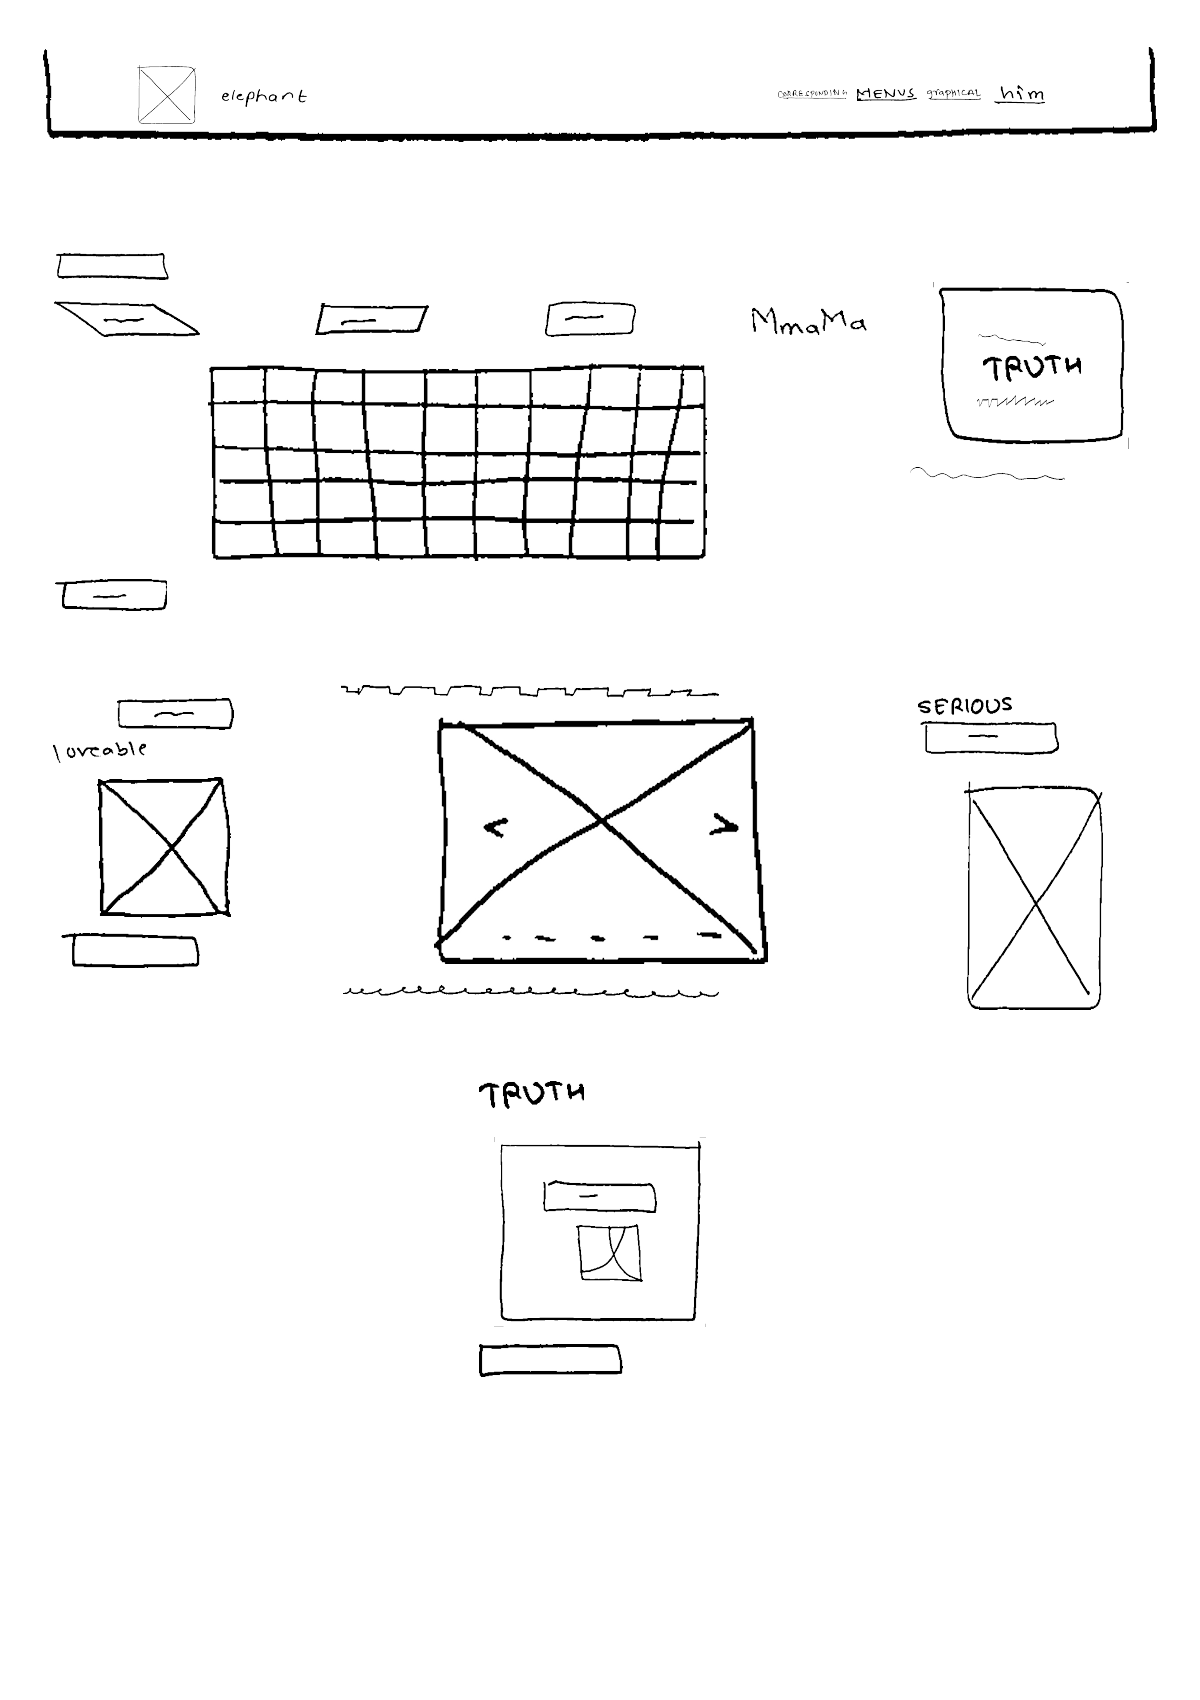
\includegraphics[width=\linewidth]{images/sample2-sketch.png}
        \caption{Sketch}
        \label{fig:s22}
    \end{minipage}
\end{figure}
\vspace{1em} 
    \pagebreak




\section{\MakeUppercase{Remaining Tasks}}


The remaining tasks are:
\begin{itemize}
    \item Using React component for flexible and various design.
    \item Integrating multi-page navigation.
    \item Extending our element pool.
    \item Enhancing the model to generalize more with the real data input code.
\end{itemize}



    \pagebreak
    
\section{\MakeUppercase{Appendices}} \label{sec:appendices}
   
    \subsection*{Appendix A: Project Schedule}
    \addcontentsline{toc}{subsection}{Appendix A: Project Schedule}
    \begin{figure}[H]
        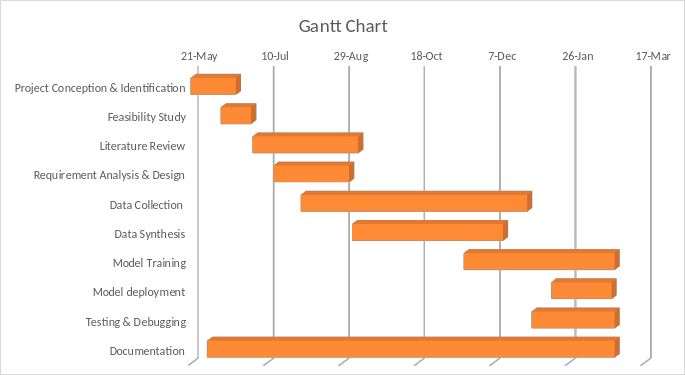
\includegraphics[width=\textwidth]{images/gantt.png}\caption{Gantt Chart}\label{fig:tabgant}
    \end{figure}

    
    \subsection*{Appendix B: \gls{dsl} Generation Rules}
    \addcontentsline{toc}{subsection}{Appendix B: DSL Generation Rules}
    \appendixnumbering{B} % For appendix Math numbering like B-1, B-2, etc.

\begin{verbatim}
1. Dictionary for Child Elements
graph={
    'root':['header','container','footer'],
    'header':['flex'],
    'nav':['navlink'],
    'logodiv':['image','text'],
    'container':['row'],
    'row':['div-3','div-6','div-9','div-12'],
    'div-3':['text','paragraph','image','card','input','button',],
    'div-6':['text','paragraph','image','card','carousel','input'
    ,'button','flex'],
    'div-9':['text','paragraph','image','card','carousel','input',
    'table','button','flex'],
    'div-12':['text','paragraph','image','card','carousel','input',
    'table','button','flex'],
    'flex':['text','button'],
    'card':['text','paragraph','image','input','button','flex'],
    'footer':['text']
}
\end{verbatim}
\begin{verbatim}
2. Rules for Child Elements
rules = {
    'root': {'inOrder': True},
    'logodiv': {'inOrder': True},
    'header':{'min':1,'max':1},
    'container': {'min': 1, 'max':3},
    'row': {'combinations':True,'0': divCombinations,
    '1':divCombinations2,'proba':0.9},
    'div-3': {'min': 2, 'max': 4},
    'div-6': {'min': 2, 'max': 4},
    'div-9': {'min': 2, 'max': 4},
    'div-12': {'min': 2, 'max':4},
    'card': {'min': 2, 'max': 3},
    'footer': {'min': 1, 'max': 1},
    'nav':{'min': 1, 'max': 5},
    'flex':{'min':2,'max':4},
}
\end{verbatim}
\begin{verbatim}
3. DSL to HTML mappings = {
    "opening-tag": "{",
    "closing-tag": "}",
    "body": "\r\n {} <style>\nmax-width: 900px;
    \nmax-height: 300px !important;\n</style>\n",
    "root": "\r\n<div class=\"root\">{}</div>\r\n",
    "header": "\r\n<header class=\"header\">{}</header>\r\n",
    "nav": "\r\n<nav class=\"nav\">{}</nav>\r\n",
    "navlink": "\r\n<a href=\"#\" class=\"navlink\">[]</a>\r\n",
    "logodiv": "\r\n<div class=\"logodiv\">{}</div>\r\n",
    "container": "\r\n<div class=\"container\">{}</div>\r\n",
    "row": "\r\n<div class=\"row\">{}</div>\r\n",
    "div-3": "\r\n<div class=\"div-3\">{}</div>\r\n",
    "div-6": "\r\n<div class=\"div-6\">{}</div>\r\n",
    "div-9": "\r\n<div class=\"div-9\">{}</div>\r\n",
    "div-12": "\r\n<div class=\"div-12\">{}</div>\r\n",
    "flex": "\r\n<div class=\"flex\">{}</div>\r\n",
    "flex-sb": "\r\n<div class=\"flex-sb\">{}</div>\r\n",
    "flex-c": "\r\n<div class=\"flex-c\">{}</div>\r\n",
    "flex-r": "\r\n<div class=\"flex-r\">{}</div>\r\n",
    "text": "\r\n<div class=\"text\">{}</div>\r\n",
    "text-c": "\r\n<div class=\"text-c\">{}</div>\r\n",
    "text-r": "\r\n<div class=\"text-r\">{}</div>\r\n",
    "paragraph": "\r\n<p class=\"paragraph\">{}</p>\r\n",
    "image": "\r\n<img src=\"placeholder.jpg\" class=
    \"image\">\r\n",
    "card": "\r\n<div class=\"card\">{}</div>\r\n",
    "input": "\r\n<input type=\"text\" class=\"input\" 
     placeholder=\"Enter text\">\r\n",
    "button": "\r\n<button class=\"button\">{}</button>\r\n",
    "button-c": "\r\n<button class=\"button-c\">{}</button>\r\n",
    "button-r": "\r\n<button class=\"button-r\">{}</button>\r\n",
    "footer": "\r\n<footer class=\"footer\">{}</footer>\r\n",
    "table": "\r\n<table class=\"table\">{}</table>\r\n",
    "carousel": "\r\n<div class=\"carousel\">{}</div>\r\n"
}
\end{verbatim}
\begin{verbatim}
4. Color Mapping for each elements = {
        'paragraph': np.array([193, 188, 192]),
        'text': np.array([255, 255, 255]),
        'button': np.array([19, 247, 47]),
        'navlink': np.array([255, 0, 0]),
        'carousel': np.array([255, 165, 0]),
        'table': np.array([165, 42, 42]),
        'input': np.array([255, 159, 252]),
        'image': np.array([0, 0, 255]),
        'header': np.array([0, 255, 255]),
        'footer': np.array([154, 128, 235]),
        'card': np.array([0, 128, 128]),
    }
    \end{verbatim}
    

\pagebreak


% References (IEEE style)
\bibliographystyle{IEEEtran}  % Use IEEE bibliography style
\bibliography{refs}
\addcontentsline{toc}{section}{References}


\end{document}
